\documentclass[book.tex]{subfiles}
\begin{document}
PC performances in the 90s were so overwhelmingly dominated by their CPU that they were simply referred to not by their brand or GPU\footnote{There were no GPU yet. The term was coined by Nvidia in 1999, who marketed the GeForce 256 as "the world's first GPU", or Graphics Processing Unit.} but by their Intel chip. If your PC had a 80386 or equivalent in it, it was a 386. If it had an Intel 80286, it was a 286. Wolfenstein was target at what was majoritarily found on people's desk: The 386s with degraded performances (yet still playable) on 286s.\\
\\
The machine can be broken down in five sub-systems parts together forming one pipeline: Input, Cpu, Ram, Video and Audio.\\
 \bigskip
\begin{figure}[H]
\centering
\includegraphics[width=\textwidth]{imgs/drawings/fun_pipeline.pdf}
%\def\svgscale{1.5}
%\input{imgs/fun_pipeline.pdf_tex}
\caption{Hardware pipeline.}
\label{fig:digraph}
\end{figure}

As I will describe, none of theses part were good for a 3D game engine although some were worse than others:

 \bigskip

\begin{figure}[H]
\centering
\begin{tabularx}{\textwidth}{ X X  }
  \toprule
  \textbf{Stage} & \textbf{Quality} \\ \bottomrule
  RAM & Bearable \\ 
  Video & Impossible \\ 
  Audio & Very Poor \\ 
  Inputs & Ok \\ 
  CPU & Impossible \\ \bottomrule
\end{tabularx}
\caption{Component quality for a game engine.}
\end{figure}

The pipeline offered a lot of resistance: hardware manufacturers had not embraced the game industry yet and it showed: PC Gaming was a niche market.\\

\section{CPU: Central Processing Unit}
  \subsection{Overview}
  The ubiquitous CPU manufacturer was Intel with its x86 line of microprocessors. The machines based on the 16 bits 80286 released in 1982 were on the decline and progressively replaced by Intel's first 32 bits processor: The 80386 which was commonly called 386 or i386. Moore's law was in full swing as seen on a MIPS\footnote{Million Instructions Per Second.} histogram:


\definecolor{skyblue1}{rgb}{0.1,0.624,0.812}
\begin{figure}[H]
\centering
  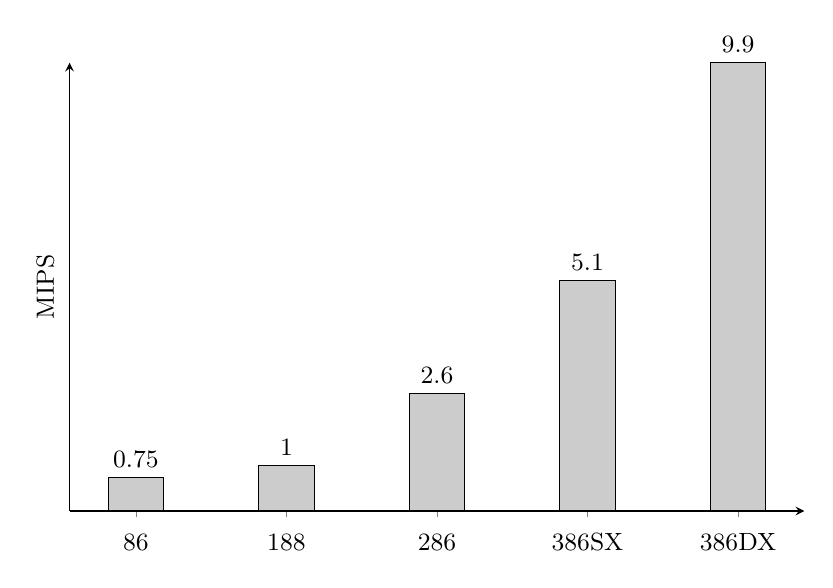
\begin{tikzpicture}[font=\small]
    \begin{axis}[
      width=0.9\textwidth,
      height=0.6\textwidth,
      ybar,
      bar width=20pt,
      ylabel={MIPS},
      ymin=0,
      ytick=\empty,
      xtick=data,
      axis x line=bottom,
      axis y line=left,
      enlarge x limits=0.11,
      symbolic x coords={86,188,286,386SX,386DX},
      xticklabel style={anchor=base,yshift=-\baselineskip},
      nodes near coords={\pgfmathprintnumber\pgfplotspointmeta}
    ]
      \addplot[fill=black!20,draw=black] coordinates {
        (86,0.75)
        (188,1)
        (286,2.6)
        (386SX,5.1)
        (386DX,9.9)
      };
    \end{axis}
    
   \end{tikzpicture}
   \caption{Processor speeds comparison.} \label{fig:mips}
 \end{figure}

 \textbf{\underline{Trivia :}} A modern processor such as the Intel Core i7 3.33 GHz operates at close to 180,000 Mips: Five orders of magnitude faster!

 \bigskip
 
 \textbf{\underline{Trivia :}} The 386SX and 386DX were identical processor. Yet the DX is twice faster than the SX thanks to a data bus between the CPU and the RAM twice as wide (32 bits vs 16 bits)!

\par

 Two other companies were producing Intel clones: AMD and Cyrix. The mediocre performances did not justify the lower cost and as a result they never gathered a significant market share. Interestingly AMD evolved to become a serious challenger while Cyrix merged with National Semiconductor in 1997.

Depite its power (at least compared to the 286), the architecture of a 386 is simple compared to 2016 Pentiums. In particular. notice the abscence of pipelineing, icache and dcache. The CPU essentially revolves around a 32 bits ALU crunching integers.

\begin{figure}[H]
\centering
  
      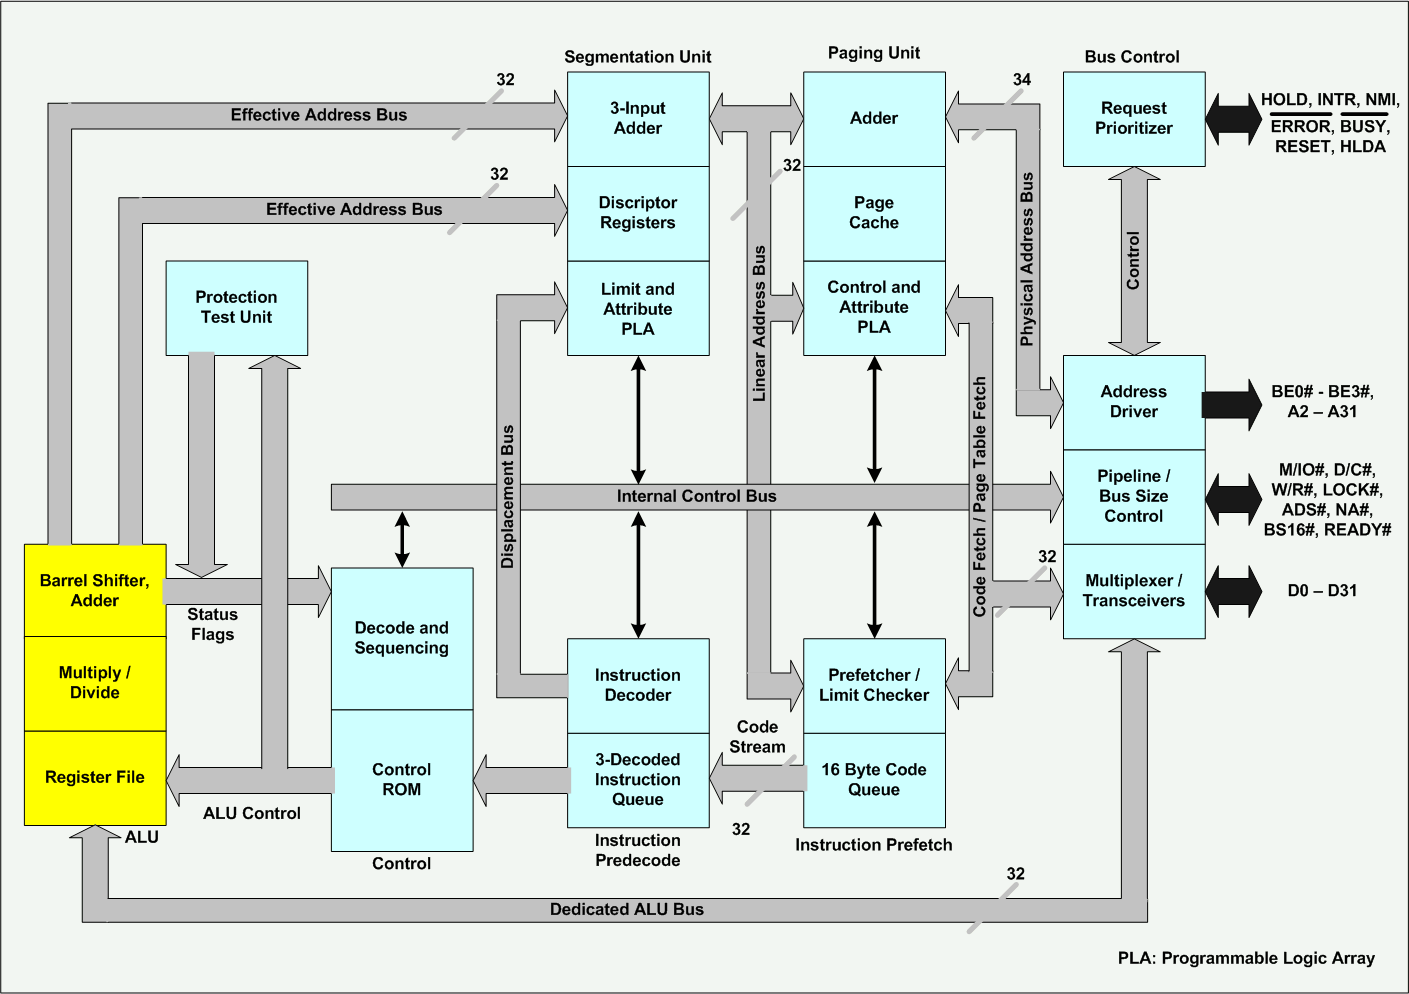
\includegraphics[width=\textwidth]{screenshots/hardware/80386DX_arch.png}
\caption{Architecture of Intel i386 DX}
\end{figure}








  \subsection{Floating Point}
  
   But is all that power necessarily useful? In order to perform all the trigonometry for a 3D game, the engine has to keep track of the fractional part of each operations. It may not look like an issue since the C programming language offers the types \codeword{float} and \codeword{double} precisely for that purpose\footnote{This is how modern 3D engine do all their calculations.}.\\
\\
It is important to understand what floating point is and how it works to fully grasp how useful it is when doing maths. In the C language, \codeword{float} are 32 bits container following the IEEE 754 standard. Their purpose is to store and allow operations on approximation of real numbers. The 32 bits are divided in three sections:\\
\begin{itemize}
  \item One bit S for the sign.
  \item Seven bits E for the exponent.
  \item Twenty four bits for the mantissa.
\end{itemize} 

\begin{figure}[H]
\centering
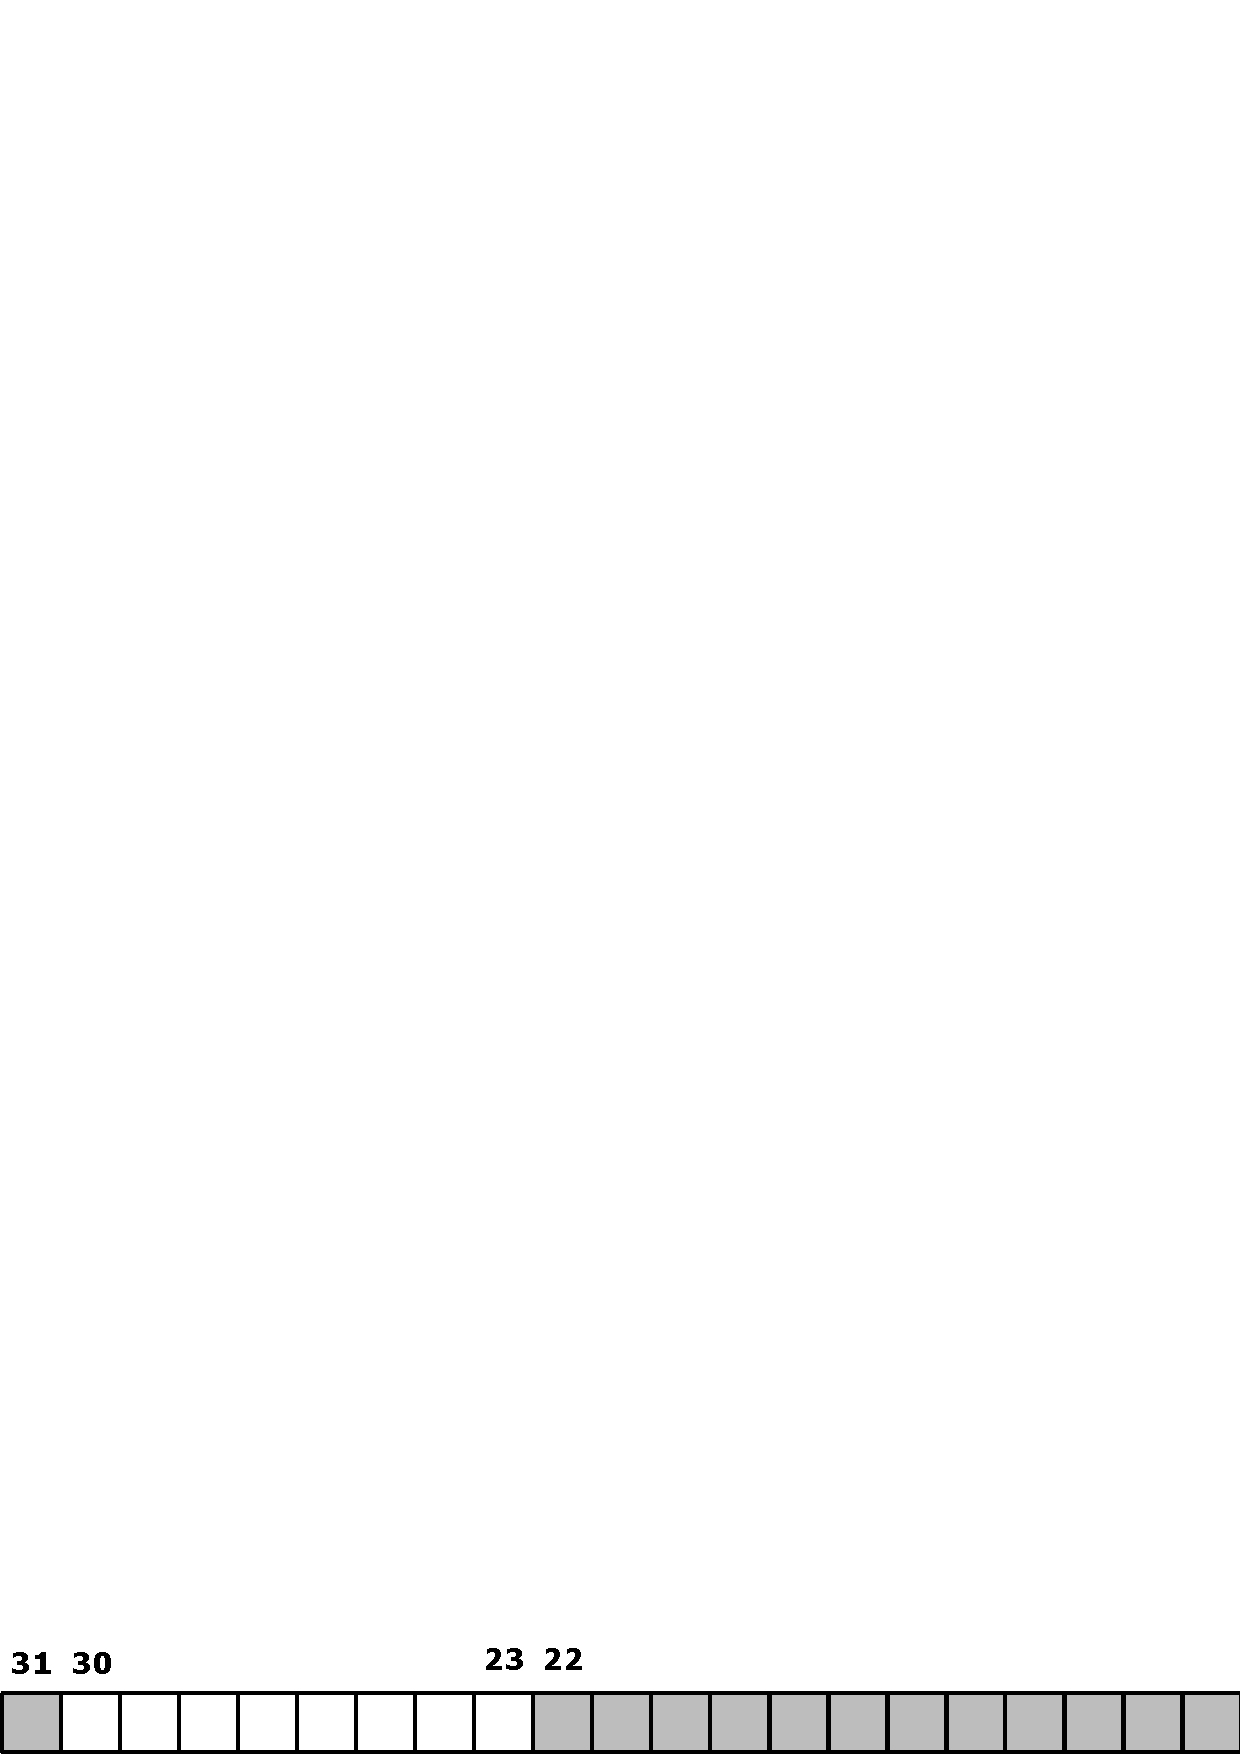
\includegraphics[width=\textwidth]{imgs/drawings/floating_point_layout.pdf}
\caption{Floating Point internals.}
\end{figure}
  \bigskip



\begin{figure}[H]
\centering
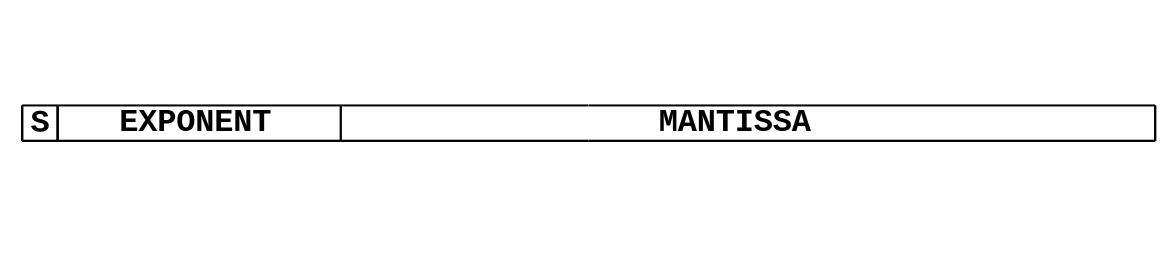
\includegraphics[width=\textwidth]{imgs/drawings/floating_point_math.pdf}
\caption{Floating Point three sections.}
\end{figure}
  \bigskip  


How numbers are stored and interpreted is usually explained with the formula in Figure \ref{eq:fp}).\

\begin{figure}[H]
\begin{equation}\label{eq:fp}
\large
(-1)^S * 1.M * 2^{(E-127)}
\end{equation}
 \caption{How everybody hates floating point to be explained to them.}
\end{figure}
\bigskip  

Although correct, this way to explain floating point usually leaves programmers completely clueless. I blame this ignoble notation for discouraging generations of programmers, scaring them to the point they never looked back to understand how floating point actually works. Fortunately, there is a better way to explain it: Instead of Exponent, think of a floating window between two consecutive power of two integers. And instead of a Mantissa think of an Offset within that window.\\ 
\par
  
\begin{figure}[H]
\centering
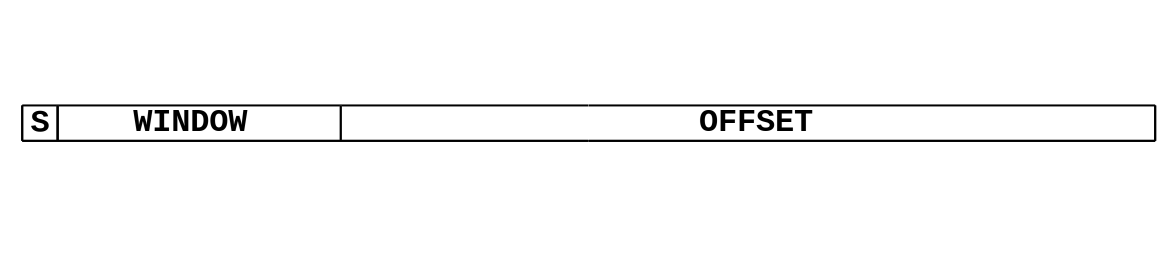
\includegraphics[width=\textwidth]{imgs/drawings/floating_point_intuitive.pdf}
\caption{Alternative Floating Point internals}
\label{fig:fp_internals}
\end{figure}
  \bigskip  
The window tells within which two consecutive power of two the number will be: [0,1], [1,2], [2,4], [4,8] and so on (up to [$2^{127}$,$2^{128}$]. The offset divides the window in 8388608 offets. With the window and the offset you can approximate a number. The window is an excellent mechanism to protect from overflowing: Once you have reached the maximun in a window (e.g: [2,4]), you can slide it right and represent the number within the next window (e.g [4,8]). It only cost a little bit of lost precision.\\
\par \bu{Trivia :} How much precision is lost ? Let's take an example with window [0,1] where 8388608 offsets give precision of $(1-0)/8388608=0.00000011920929$. In the window [2048,4096] the precision is $ (4096-2048)/8388608=0.0002$.\\
\par

Figure \ref{fig:fp_internals_window} illustrates how the number 6.1 would be encoded with the window starting at 4 (and therefore spanning up to next power of two: 8). The offset about half way down the window.

\begin{figure}[H]
\centering
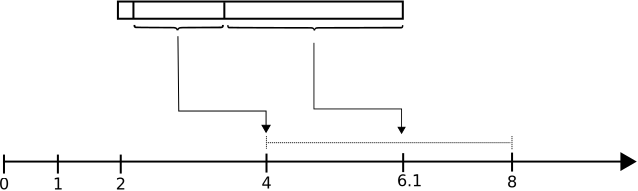
\includegraphics[width=\textwidth]{imgs/drawings/floating_point_window.pdf}

\caption{Value 6.1 approximated with floating point}
\label{fig:fp_internals_window}
\end{figure}
  \bigskip
  
Here is a detailed example which calculate the floating point representation of the number 3.14.
\begin{itemize}
 \item The number 3.14 is positive  $\rightarrow S=0$.
 \item The number 3.14 is between the power of two 2 and 4 so the floating window must start at $2^1$  $\rightarrow E=128$.
 \item Finally there are $2^{23}$ offsets available so 3.14 is at $\frac{4-3.14}{2} = 0.43 $. The mantissa/offset $\rightarrow M = 2^{23}*0.43 = 4781506$
\end{itemize}

Which in binary translate to:

\begin{itemize}
\item S = 0.
\item E = 10000000
\item M = 1001000111101111000011
\end{itemize}

\begin{figure}[H]
\centering
\includegraphics[width=\textwidth]{imgs/drawings/floating_point_layout_pi.pdf}
\caption{Floating Point internals}
\label{fig:fp_internals}
\end{figure}
  \bigskip

The value 3.14 is therefore approximated to 3.140000104904175.\\

The corresponding value with the ugly and useless formula:

\begin{equation}
3.14 = (-1)^0 * 1.57 * 2^{(128-127)}
\end{equation}

\bigskip

And finally the graphic representation with window and offset:\\

\begin{figure}[H]
\centering
\includegraphics[width=\textwidth]{imgs/drawings/floating_point_window_pi.pdf}

\caption{3.14 window and offset.}
\label{fig:fp_internals}
\end{figure}
  \bigskip

For a 3D engine floating points are very handy: They can represent very small values and huge ones while keeping track of fractional part of a number and also protecting from overflow by floating the window when necessary.\\
\\
They are neat but computational intensive: In order to add, subtract, multiply or divide two numbers, they have to be expressed with the same window. Which mean converting one number to the representation used by the other usually with higher precision than 32 bits (typically 80 bits on Intel FPUs).\\
\\
This is not a problem when everything is hardwired within an hardware floating point unit...but it is a big problem for the 386: \emph{They do NOT not have a hardware Floating Point Unit}. If found in the code, these operations are emulated in software by the compiler, resulting in terribly slow processing. So slow they are not usable for anything real-time.\\ 
\par


 \textbf{\underline{Trivia :}} Since floating point units where so slow, why did the C language end up with a \cw{float} and \cw{double} types ? The machine used to invent the language (PDP-11) did not have a floating point unit but the manufacturer (DEC) had promised to Dennis Ritchie and Ken Thompson the next model would have one\footnote{The Development of the C Language by Dennis M. Ritchie}. Being astronomy enthusiasts they decided to add those two types to their language. Had they decided not to, C and C++ would have never enjoyed the same popularity!\\
\par

\textbf{\underline{Trivia :}} Some PCs did have hardware FPU. Intel marketed them as "Math CoProcessor". Intended to scientists, performances were average and price outrageous\footnote{\$200 in 1993 equivalent to \$350 in 2016}. As a result, sales were mediocre:\\
\begin{figure}[H]
\centering
  \shadowbox{
      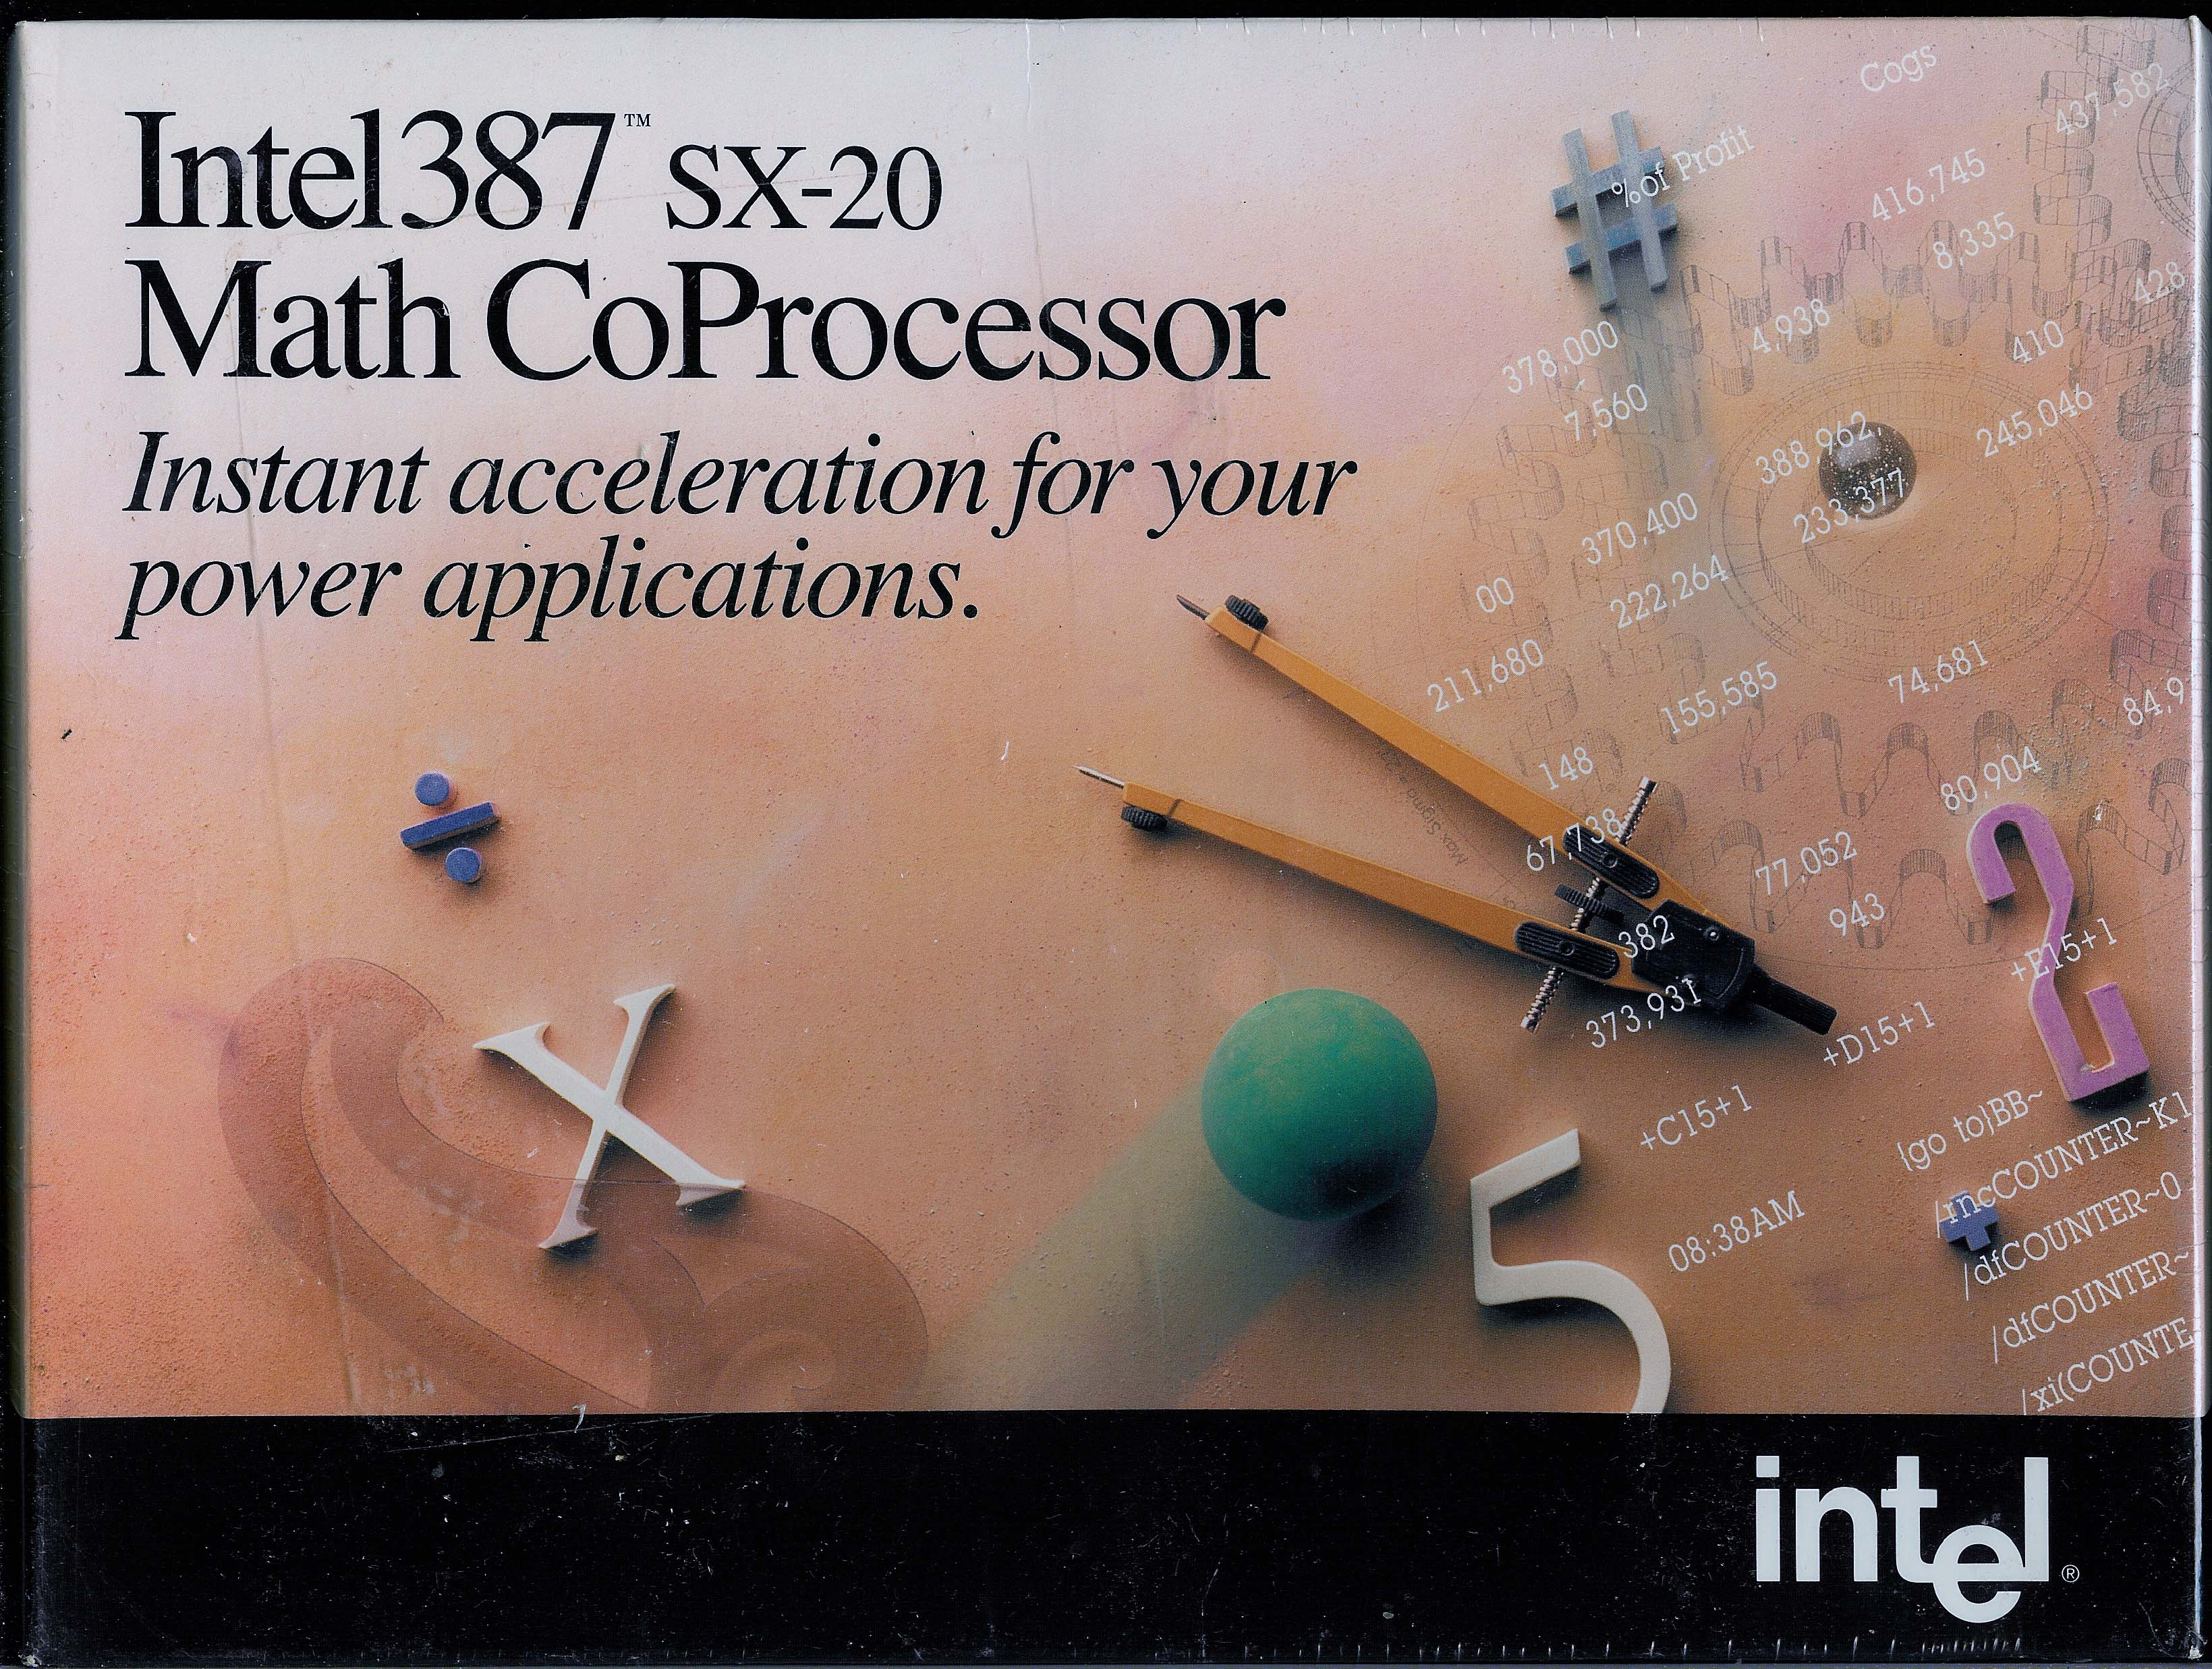
\includegraphics[width=\textwidth]{screenshots/BOX_IntelBOX387SX20.jpg}
  }
\caption{Intel 1991 ad for "Math CoProcessor".}
\label{fig:fp_internals}
\end{figure}



\par
A game engine designed was stuck in an awkward situation with two half solutions to his problem: \cw{int}(integer) operations which were fast but not accurate enough and \cw{float} operations whcih were accurate but not fast enough!
  















\section{RAM}
A 386 can operate in two modes:\\
\par
\begin{itemize}
  \item The new\footnote{Well, in 1991 it was new!} Protected Mode with  32 bits registers and 24 bits address bus wide offering up to 16 MB of flat RAM protectable with a MMU\footnote{Memory management Unit}.
  \item The backward compatible Real Mode. Available only to allow old software to run. This memory model replicated how the Intel 8086 CPU from the 1976 operated: 16 bits registers, 20 bits address bus giving 1MB addressable RAM with an awful segmented addressing system. 
\end{itemize}
For compatibility reasons all PCs starts in Real Mode. You may assume that programmers of the 90s promptly switched the CPU to Protected Mode to unleash the full potential of the machines and ditch the 20 years old Real Mode. Unfortunately, there was a major obstacle between this nice feature and the programmer. The infamous operating system: MS-DOS 5.0 by Microsoft Corporation.
  






  \subsection{DOS limitations}
  Microsoft Corporation highly valued the applications running on their operating systems. As an excellent business priority, they were adamant to never ever break anything with a new system.  Since many applications were written during the 80s on machine having only Real-Mode, DOS 5.0 kept running that way and as a result its routines and system calls were incompatible with Protected Mode. This created an awkward situation where the \emph{de-facto} operating system delivered with every machine sold prevented programmers from using Protected Mode. Developers were forced to ignore all the neat features of their 1992 PC and use the machine like it was a very fast Intel 8086 CPU from 1976.

\bigskip

 \textbf{\underline{Trivia :}} One year earlier, in 1991, a student from the University of Helsinki started working on a hobby, "nothing big", of his : An operating system able to use the CPU in Protected Mode taking advantage of the MMU and the 32 bits registers. It would become Microsoft worse nightmare: Linus Torvalds had just started what would become Linux.



  \subsection{The infamous Real Mode: 1MB RAM max}
  Protected mode was unavailable. What had the Real-Mode to offer ? Essentially a trip back in time to 1976: A 20 bits wide address bus offering only 1MB of addressable RAM. No matter how much memory was installed on the machine in 1992, only 1MB could be addressed. And to top it all, addressing had to be done not with the 32 bits registers available but by combining two 16 bits register together: One was the segment, the other an offset within that segment. Hence the name: '16 bits programming'.

  \bigskip
Here is how the memory was layout: \\
\begin{itemize}
\item From 00000h to 003FFh : the Interrupt Vector Table.
\item From 00400h to 004FFh : BIOS data.
\item From 00500h to 005FFh : command.com+io.sys.
\item From 00600h to 9FFFFh : Usable by a program (about 620KB in the best case). 
\item From A0000h to FFFFFh : UMA (Upper Memory Area): Reserved to bios ROM, video card and sound card mapped I/O.
\end{itemize}

\begin{figure}[H]
\centering
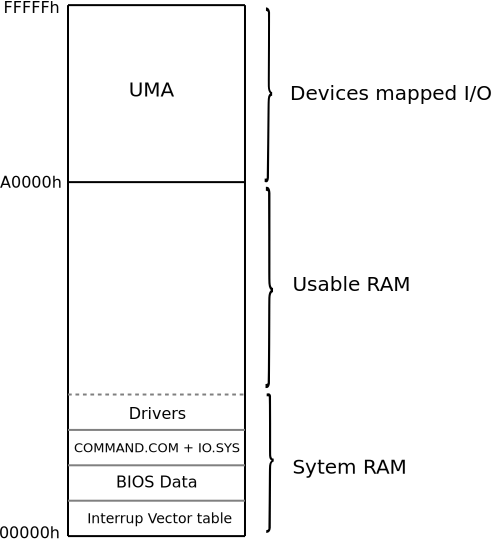
\includegraphics[width=\textwidth]{imgs/drawings/real_mode.pdf}

\caption{3.14 window and offset.}
\label{fig:fp_internals}
\end{figure}


As a result, out of the original 1024KB, only 640KB (called Conventional Memory) were usable. 384KB were reserved for the UMA\footnote{Upper Memory Area} and every single driver installed (\codeword{.SYS} and \codeword{.COM})  took away from the remaining 640KB.

\bigskip

\textbf{\underline{Trivia :}}  In France people had to load KEYBFR.SYS driver so their AZERTY keyboard keys would be properly mapped. The driver consumed a whopping 5KB of Conventional Memory. Needless to say French people had a strong incentive to learn that god mode was iddAd\footnote{Invincibility mode in Doom is iddQd on a querty keyboard but iddAd on an azery keyboard without the French driver loaded.}.\\
\\

\subsection{The infamous Real Mode: 16 bits Segmented addressing}
386 has 32 bits registers but Real Mode cannot use them for addressing (or even operations as a matter of facts). Everything has to be done by combining two 16 bits registers as seen in Figure \ref{fig:register_comb_to_20_bits}. There are two kinds of pointers: \cw{near} and \cw{far}. A \cw{near} pointer is 16 bits and considered \emph{fast} because it can be used as is (but it only allows the IP to \cw{jmp} 16K in the code section). A \cw{far} pointer allows a \cw{jmp} anywhere but it is slower since a 16 bits segment register has to be shifted left 4 bits and combined with an other 16 bits offset register to form a 20 bits address:\\
\begin{figure}[H]
\centering
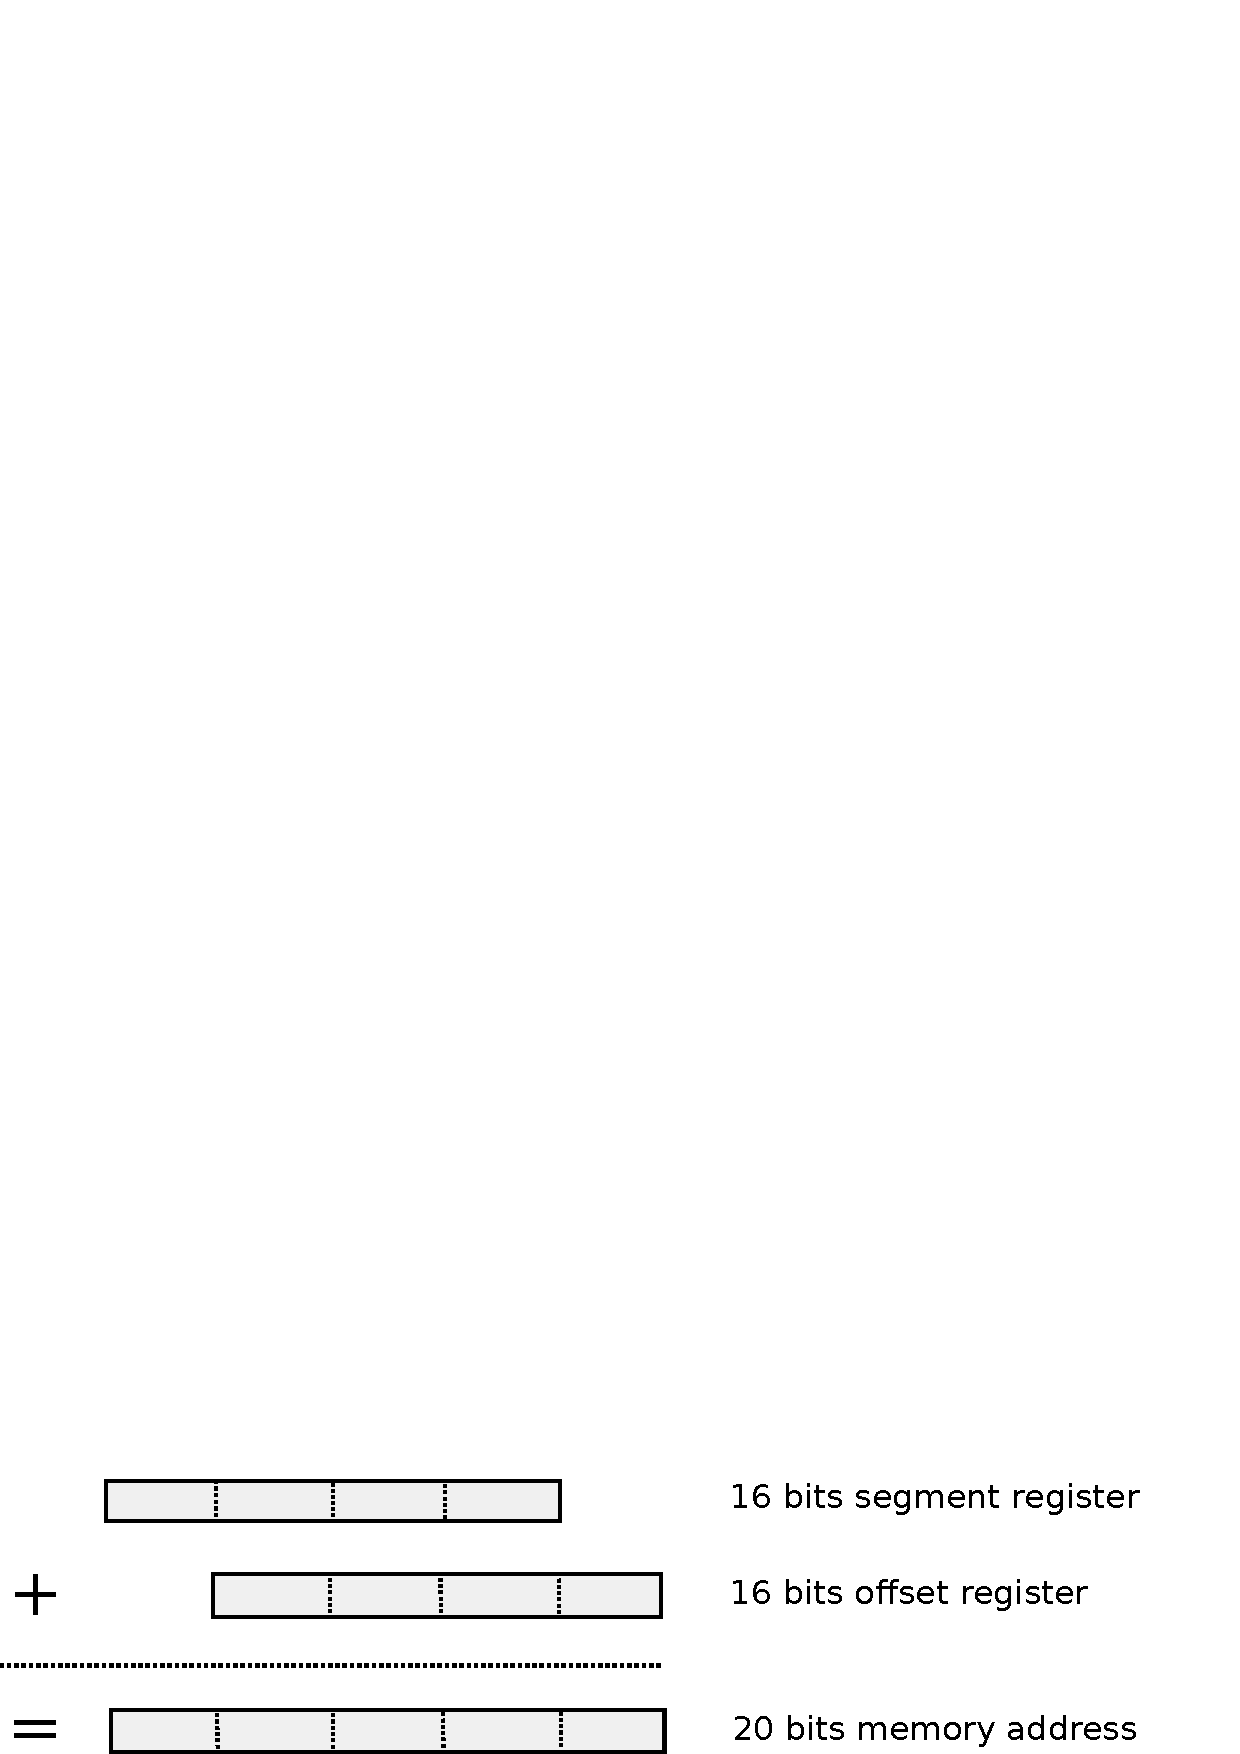
\includegraphics[width=\textwidth]{imgs/drawings/register_combination_20_bits_address.pdf}
\caption{How registers are combined to address memory.}
\label{fig:register_comb_to_20_bits}
\end{figure}
That may not sound too bad but in practice this segmented addressing led to many issues.\\
\par 
The least problematic was about the language C: Since it was invented on a flat memory machine, it had to be augmented by compiler manufacturers. That is how the \codeword{near} and \codeword{far} keywords came to existence. To build pointers, a set of macro would be provided, respectively \codeword{FP\_SEG} and \codeword{FP\_OFF}. That was an ugly wart on the beautiful C but that was manageable. And of course \cw{libc} was also different: \cw{malloc} returns \cw{near} and can therefor only allocate 64K. To allocate more \cw{farmalloc} is used.\\
\\
The really big issue however was how two pointers referring to the same address could fail an equality test: In this model, the 1MB of RAM is divided in 65536 paragraphs by the segment pointer. So a paragraph is 16 bytes but an offset can be up to 65536 which result in a maze of overlaps! See the following example:\\
\par
Pointer A defined as:\\
\par
\begin{minipage}{\textwidth}
\lstinputlisting[language=C]{code/pointer_madness1}
\end{minipage}

\bigskip

Pointer B defined as:\\
\par
\begin{minipage}{\textwidth}
\lstinputlisting[language=C]{code/pointer_madness2}
\end{minipage}

\bigskip

Pointer C defined as:\\
\par
\begin{minipage}{\textwidth}
\lstinputlisting[language=C]{code/pointer_madness3}
\end{minipage}

As defined A, B and C all points to the same memory location however they would fail a comparison test in the following code.\\

\begin{minipage}{\textwidth}
\lstinputlisting[language=C]{code/pointer_madness.c}
\end{minipage}
Would output:\\

\begin{minipage}{\textwidth}
\lstinputlisting{code/pointer_madness_output.txt}
\end{minipage}
\par

You also have to be careful about pointer arithmetic e.g: A \cw{far} pointer increment only increment the offset, not the segment. If you iterate on an array more than 64KB you can end up wrapping around! You could use \cw{int huge*} pointer to make pointer arithmetic work but...nobody wants to go there.




  \subsection{Extended Memory}

The 20 bits address bus of Real Mode limited the addressable RAM to 1MB. But machines of 1992 came equipped with more, typically 2MB and even sometimes 4MB. The workaround at the time was to install special drivers that would open a window beyond the addressable RAM as shown in Figure \ref{fig:ems_xms_layout}.

\begin{figure}[H]
\centering
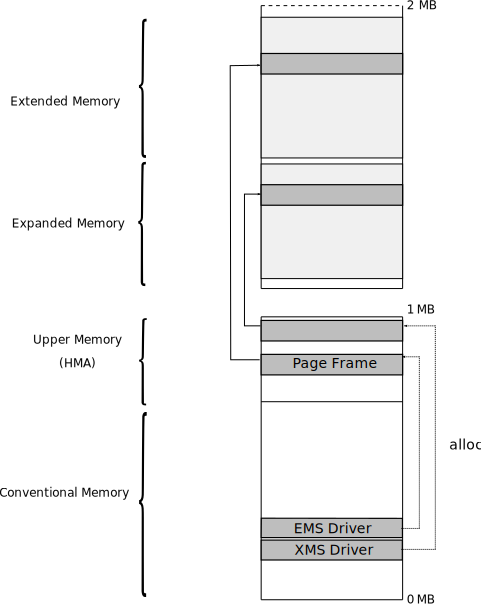
\includegraphics[width=\textwidth]{imgs/drawings/expanded_ram.pdf}
\caption{Expanded memory layout}
\label{fig:ems_xms_layout}
\end{figure}
With this system, programmer could map part of the upper memory to RAM located beyond the addressable space.
Unfortunately once again, nothing was standardized. Users could load different drivers providing different memory mapping systems:
\begin{itemize}
\item Expanded Memory Specification (EMS) drivers: EMM368.SYS.
\item eXtended Memory Specification (XMS) drivers: HIMEM.SYS .
\end{itemize}

Or they could decide to load no drivers at all at startup and not use any of the RAM beyond 1MB.\\
\par
\textbf{\underline{Trivia :}}  This 640KB barrier was a big issue. Many customer could not understand why, even though they had many (extremely expensive\footnote{In 1992, 4MB of RAM cost \$149 which ajusted to inflation would be \$256 in 2016.}) megabytes of RAM installed on their machine, some game would refuse to start up claiming "Not enough memory". id Software had to publish an explanation (Appendix "\nameref{chap:barrier640}") along with the game to make it clear that it was not their fault.\\

\textbf{\underline{Trivia :}}  As of 2014, thirty five years after the introduction of the 8086, most PC in the world still start in Real Mode. A bootloader switch them to protected mode, load the kernel and then real startup can begin. Mac computers don't have this problem.

\bigskip
To learn more about EMS be sure to read Edward Mendelson's excellent article: . "A Slot Full of RAM"\footnote{PC Mag, (1989-12-12).}. If you are really hardcore, you can also check out XMS programming reference:\footnote{eXtended Memory Specification (XMS) July 19, 1988.}\\
\par

\subsubsection{Impossible to love}
These two sections conclude on Intel CPUs. If you are puzzled you are not alone. Over the years I came around many ways to describe this madness but two particularely stand up:\\
\par
 \begin{fancyquotes}
   The i386 \lbrack...\rbrack an architecture that is difficult to explain and impossible to love.\\
   \par
\textbf{David Patterson \& John Hennessy - Computer Organization and Design.}
 \end{fancyquotes}\\
\par
And:
\par
 \begin{fancyquotes}
    That sounds odd, but Intel built it, Microsoft wrote it, and DOS grew up around it.\\
   \par
\textbf{Eccles-Jordan Trigger - Codeproject.com.}
 \end{fancyquotes}\\



\par
\bu{Trivia :} 640KB was all a game could have. But people writing compilers got clever. Strike Commander (a very famous flight arcade game released in 1993) executable is 745KB which obviously doesn't fit in. The trick was to use a technique of "overlays". The compiler inserted instructions at compile time to detect when the IP was about to beyond a page. These insctructions swaped code segment from RAM to CPU and issued a \cw{jmp} to reset the CPU at the beginning of the new code. To get a better idea of how it works: Think of Gromit seating on top of the train and inserting rails as the machine is moving forward at full speed.

















\section{Video}

PCs were connected to CRT monitors: Big, heavy, small diagonal, cathodic ray based with curved surface screens. Most monitors had a 13" diagonal with a 4:3 aspect ratio. To give you an idea of the size, Figure \ref{fig:int_layout} shows a comparison between a 13" CRT from 1992 and a 23" LCD display from 2014.\\

\begin{figure}[H]
\centering
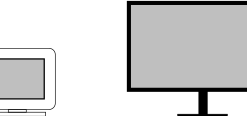
\includegraphics[width=\textwidth]{imgs/drawings/crt_lcd.pdf}
\caption{CRT (left) vs LCD (right)}
\label{fig:lcd_vs_crt}
\end{figure}

\textbf{\underline{Trivia :}} How big and heavy could a CRT be ? The InterView 28hd96 by Integraph weighted 45kg (99.5lb). For comparison, a modern DELL LCD 27" weights 7.8kg (17lb).\\
\\
The main issue in this system is that CRT are analogic system while computers are digital. An interface is needed between the two and it came as a serie of chipsets called "Adapters". 

  \subsection{History}

The first adapter of the family was released in 1981. The Monochrome Display
   Adapter (\codeword{MDA}) was monochrome with low resolutions but it had the merit to be on every PC sold. Many other systems followed over the years, always preserving backward compatibility like it was the tradition at the time:
\bigskip
  
 \begin{figure}[H]
\centering  
\begin{tabularx}{\textwidth}{ X  Y }
  \toprule
  \textbf{Name} &  \textbf{Year Released} \\
  \toprule \codeword{MDA}
   (\textbf{M}onochrome
   \textbf{D}isplay
   \textbf{A}dapater) & 1981 
   \\ \codeword{CGA}
   (\textbf{C}olor
   \textbf{G}raphics
   \textbf{A}dapter) & 1981 
    \\ \codeword{EGA}
   (\textbf{E}nhanced
   \textbf{G}raphics
   \textbf{A}dapter) & 1985
   \\ \codeword{VGA}
   (\textbf{V}ideo
   \textbf{G}raphics
   \textbf{A}rray)  & 1987
    \\
  \toprule
\end{tabularx}
\caption{Video interface history.}\label{fig:vga_history}
\end{figure}

Each iteration added new features and in 1991 the ubiquitous graphic system was the VGA\footnote{Video Graphic Adapter}. All video cards purchased had to follow the standard started by IBM. The universality of that system was a two edged sword: On one side developers had to program for one graphic system only. But on the other side, there was no escape to the shortcoming of the Adapter.\\

\begin{figure}[H] 
  \centering 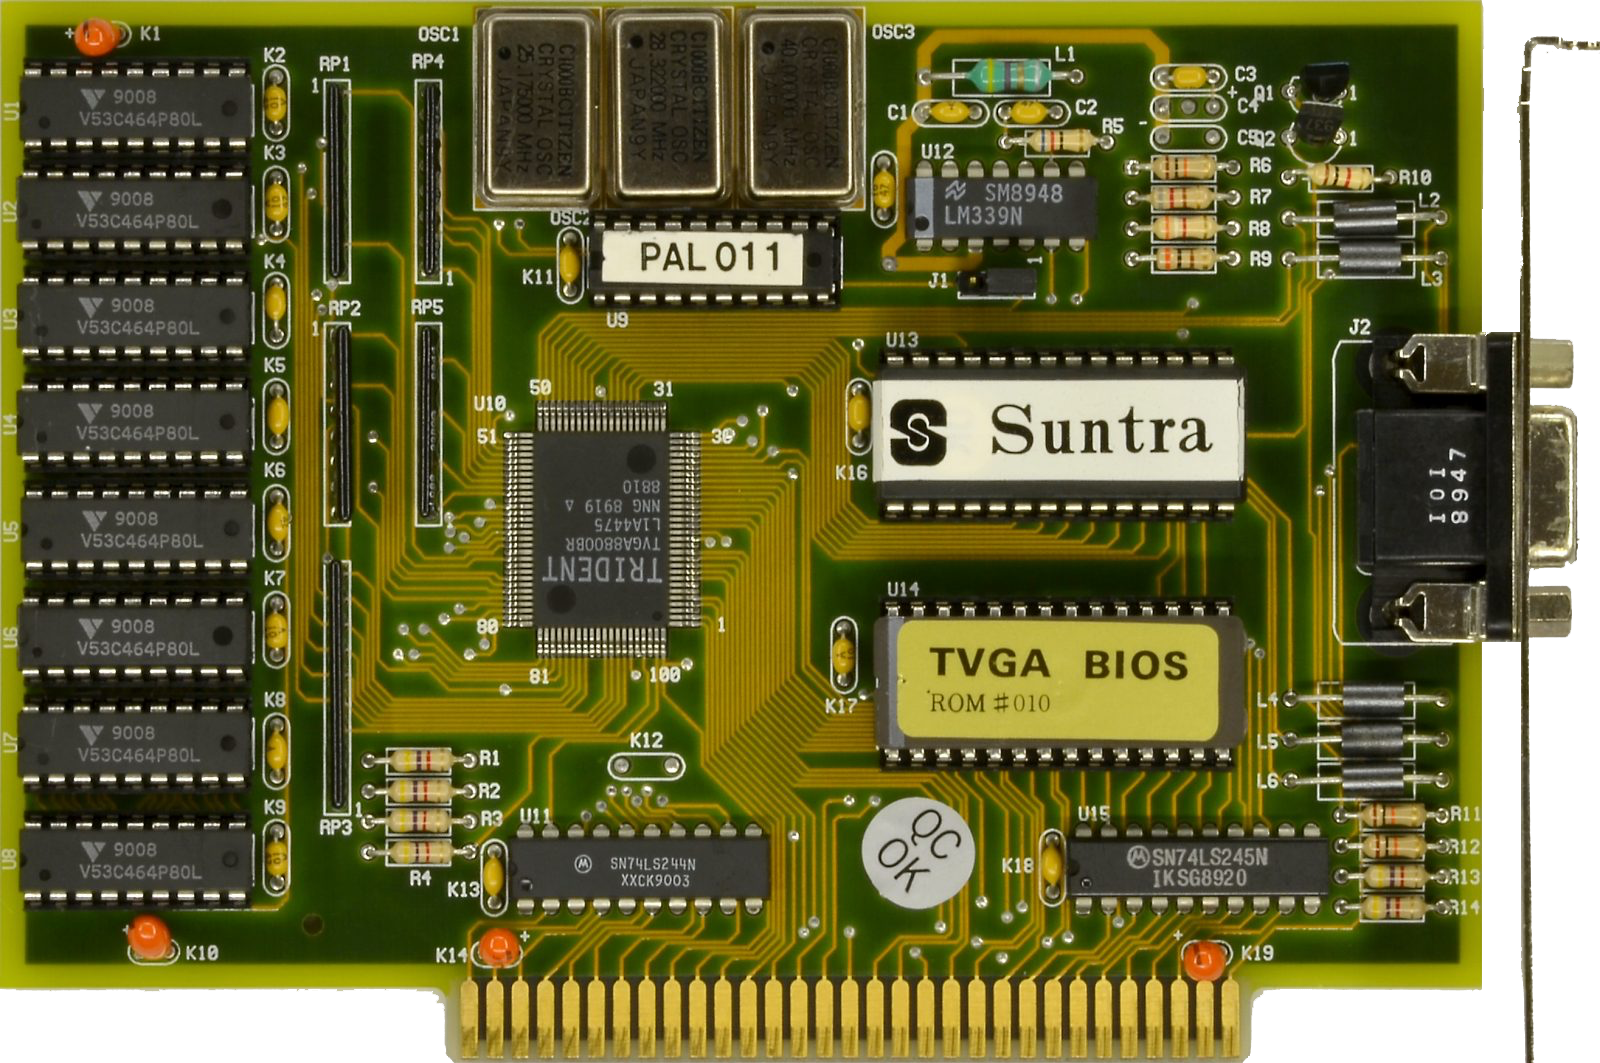
\includegraphics[width=\textwidth]{screenshots/hardware/suntra_trident_tvga8800br.png} 
  \caption{A VGA card Trident 8800 (8 bits ISA). Courtesy of \cw{vgamuseum.info}.}
\end{figure}
\par
\begin{figure}[H] 
  \centering 
  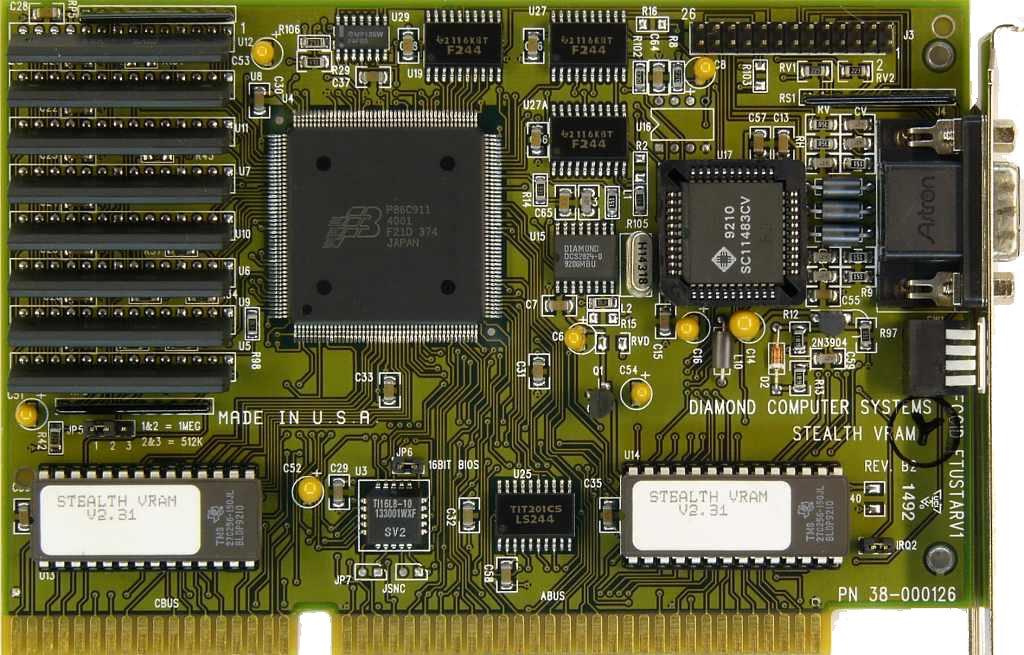
\includegraphics[width=\textwidth]{screenshots/hardware/diamond_stealth_vram_revb2.png} 
  \caption{A VGA card Diamond Stealth (16 bits ISA). Courtesy of \cw{vgamuseum.info}.}
\end{figure}
\bu{Trivia :} There was no GPU market back then. Since all video cards "only" had to be VGA compatible and have 256KB of RAM, most people just bought the cheapeast thing available. Note however that some cards only had a 8 bits ISA bus connector (like the trident) and some had an ISA 16 bits connector like the Diamond which twice as fast.\\
\par




\subsection{VGA Architecture}

The VGA can be summarized as three major systems :

\begin{itemize}
\item The Graphic Controller and Sequence Controller controlled how the VGA RAM was accessed (interface CPU-VRAM).
\item The framebuffer (the VRAM) made of not one memory bank of 256KB but four memory banks of 64KB.
\item The CRTC Controller and the DAC (Digital To Analog Converter) took care of converting the Palette indexed framebuffer to RGB and then to analogic signal (interface VRAM-CRT).
\end{itemize}

The most surprising part of the architecture is obviously the framebuffer. The first reaction of any engineer would be to ask themselves: Why four small fragment banks instead of one big linear one ?\\
\\
The first part of the explanation comes from backward compatibility: The version before VGA, the EGA had only 64KB of RAM. It was very easy to design a backward compatible system that used only one bank of 64KB.\\
\\
But the real reason was physical limitations and the need for a minimum bandwidth: A CRT running at 70Hz and displaying 640x480 needed a pixel every 1/(640*480*60)th of a second . Since the VGA is palette based, one pixel is one byte [0-255] translated to a 888 RGB color. So that divides bandwidth by three. But you still need one byte each 54ns...and unfortunately RAM access time was 200ns: Not nearly fast enough\footnote{Computer Graphic: Principles and Practice 2nd Edition, page 168} to refresh the screen at 70hz. If latency could not be reduced, the throughput could still be improved by accessing four banks at the time. The memory banks read in parallel had an amortized latency of 200/4 = 50ns/pixel which was fast enough.


\begin{figure}[H]
\centering
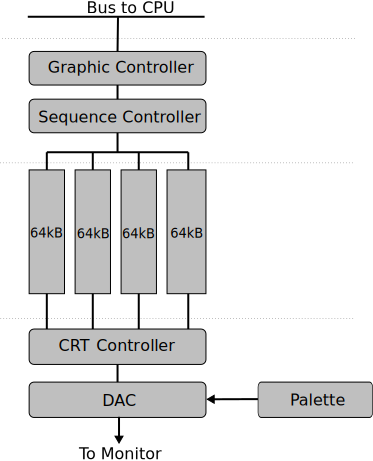
\includegraphics[width=\textwidth]{imgs/drawings/vga.pdf}
\caption{Video Graphic Array Architecture.}
\label{fig:vga_arch}
\end{figure}




\subsection{VGA Planar madness}

Four memory banks granted enough throughput to reach high resolutions. The price was complexity of programming acknowledged by even the best programmers of the time:\\

 \begin{fancyquotes}
   Right off the bat, I'd like to make one thing perfectly clear: The VGA is hard-sometimes very hard-to program for good performance.
 \bigskip \\
\textbf{Michael Abrash - Graphic Programming Black Book}
 \end{fancyquotes}
 \\
\par
The problem with this design is that programmers did not have a linear framebuffer. In order to write four pixesl next to each others on a line, a developer has to write one pixel in each bank. Each of these banks were located at the same memory address. It was a mess better illustrated with the following drawing:\\
\par
\begin{figure}[H]
\centering
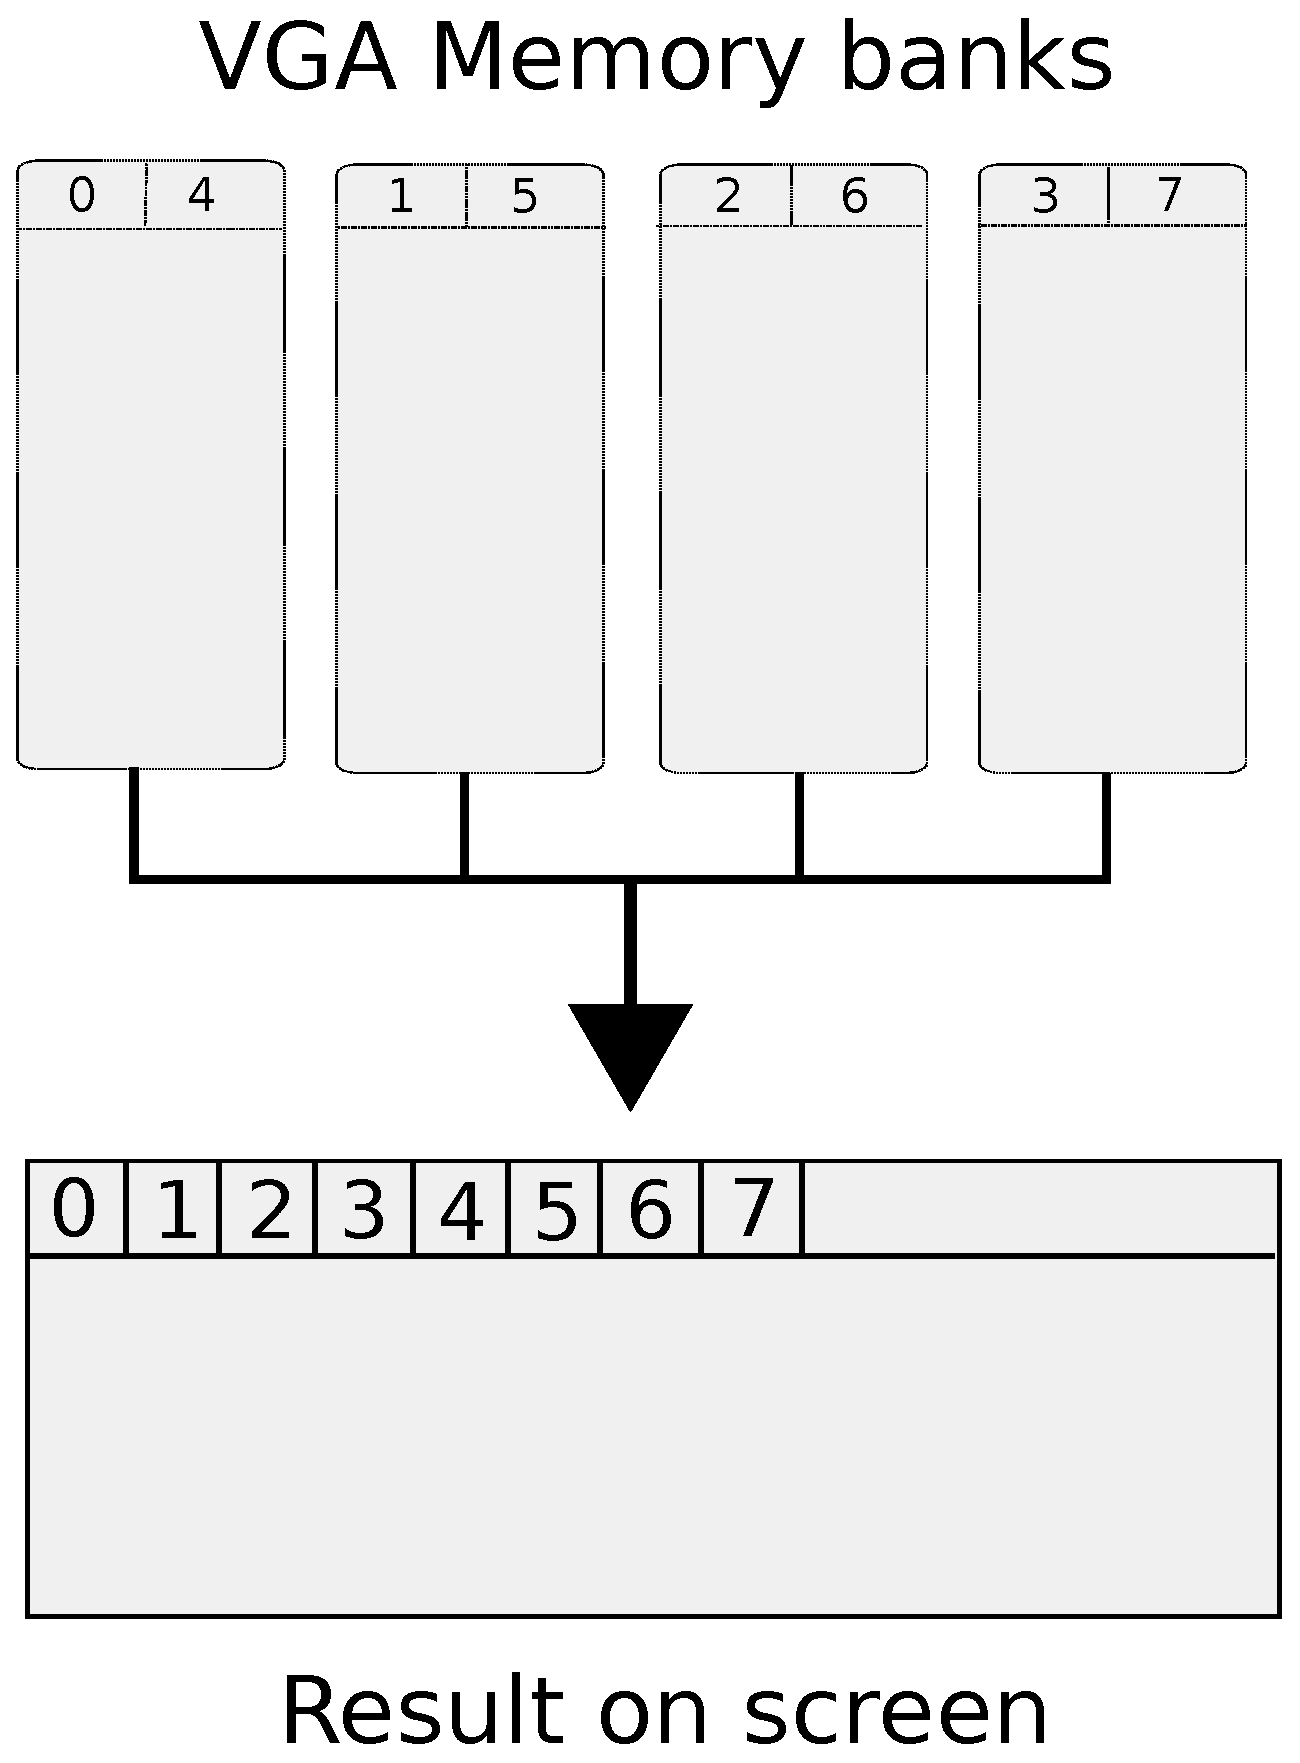
\includegraphics[width=\textwidth]{imgs/drawings/vga_ram_screen_layout.eps}
\caption{Video Graphic Array Architecture.}
\label{fig:vga_arch}
\end{figure}


 

 

\par
To configure this mess of planes and circuitry, the four controllers had a set of 300 poorly documented registers to setup. Needless to say few programmers got to dive in the internal of this thing. My first drawing of the VGA was actually deceiving: The register system and architecture of the VGA was hell as confirm the diagram from IBM VGA Reference:\\
 \begin{figure}[H]
\centering
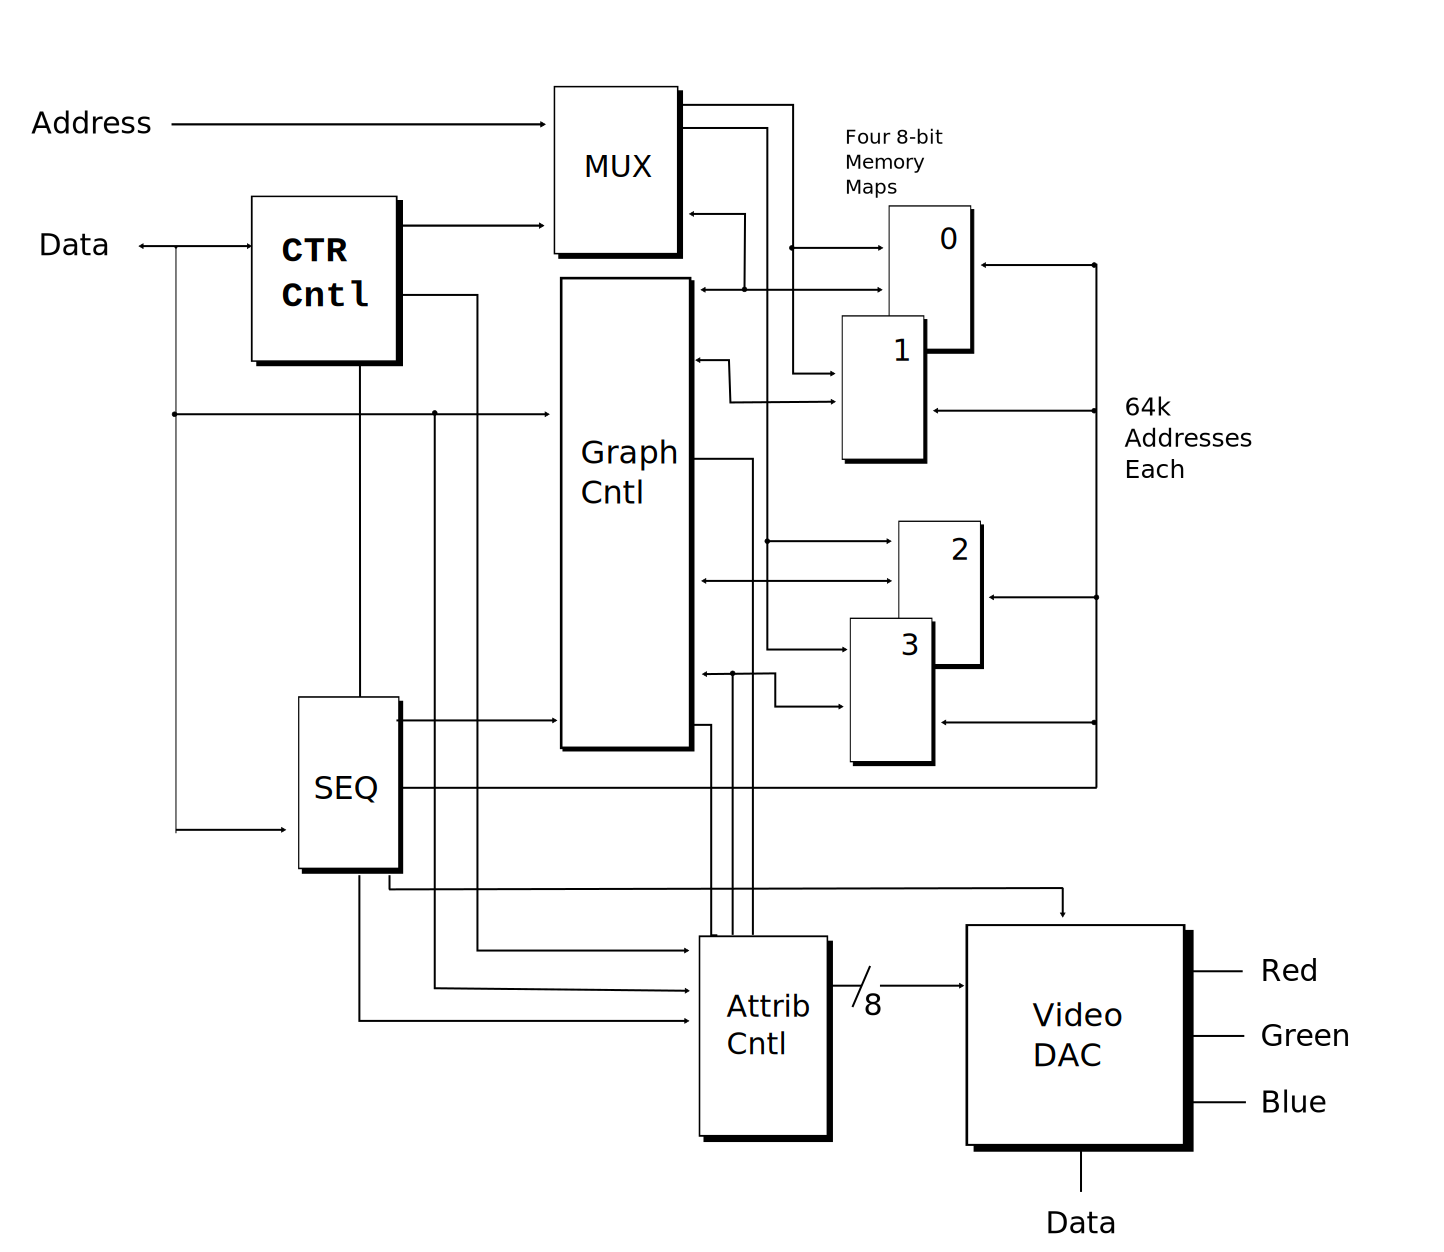
\includegraphics[width=\textwidth]{imgs/drawings/ibm_vga.pdf}
\caption{IBM's VGA Documentation}
\label{fig:ibm_vga}
\end{figure}

\bigskip



Luckily IBM provided routines to initialize all the registers via one simple BIOS call: 15 preset configurations (called "mode") with an associated resolution, color numbers and memory layout.

\subsection{VGA Modes}

The BIOS could be called to have the VGA configured with preset registers.

\begin{figure}[H]
\centering
\begin{table}[H]
\begin{tabularx}{\textwidth}[c]{llllr}
\hline
\textbf{Mode} & \textbf{Type} & \textbf{Format} & \textbf{Colors}          & \multicolumn{1}{l}{\textbf{Segment}} \\ \hline
0             & text          & 40x25           & 16 gradient (monochrome) & b800h                                \\ \hline
1             & text          & 40x25           & 16                       & b800h                                \\ \hline
2             & text          & 80x25           & 16 gradient (monochrome) & b800h                                \\ \hline
3             & text          & 80x25           & 16                       & b800h                                \\ \hline
4             & CGA Graphics  & 320x200         & 4                        & b800h                                \\ \hline
5             & CGA Graphics  & 320x200         & 4 gradient (monochrome)  & b800h                                \\ \hline
6             & CGA Graphics  & 640x200         & 2                        & b800h                                \\ \hline
7             & MDA text      & 9x14            & 3 gradient (monochrome)  & b000h                                \\ \hline
0Dh           & EGA graphic   & 320x200         & 16                       & A000h                                \\ \hline
0Eh           & EGA graphic   & 640x200         & 16                       & A000h                                \\ \hline
0Fh           & EGA graphic   & 640x350         & 3                        & A000h                                \\ \hline
10h           & EGA graphic   & 640x350         & 16                       & A000h                                \\ \hline
11h           & VGA graphic   & 640x480         & 2                        & A000h                                \\ \hline
12h           & VGA graphic   & 640x480         & 16                       & A000h                                \\ \hline
13h           & VGA graphic   & 320x200         & 256                      & A000h                                \\ \hline
\end{tabularx}
\end{table}
\caption{VGA Modes available from BIOS.}\label{fig:vga_modes}
 \end{figure}
 
 Programmers referenced VGA modes by their ID. It was a common thing to see tutorial about Mode 12h or Mode 13 which were the two most appealing mode for game programming.


 \subsection{VGA Programming: Memory mapping}
To write to the VRAM the 1MB address space maps 64KB starting as indicated in table \ref{fig:vga_modes}. So a dev had from 0xA000 to 0x1A000 available. The immediate question is "How does one write to 256KB of RAM with only 64KB ?". The answer is: Banking. Write and Read operation are routed based on a mask.\\
\par
 \begin{figure}[H]
\centering
  
      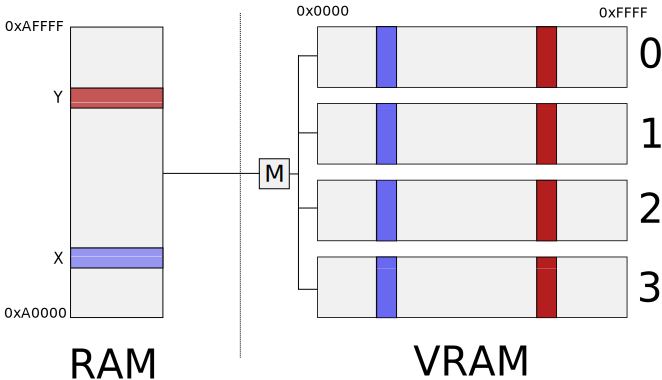
\includegraphics[width=\textwidth]{imgs/drawings/ram_to_vga_mapping.pdf}
    
\caption{Mapping PC RAM to VGA banks.}
\end{figure}



 

 \subsection{VGA Programming: Mode 12h}
 This mode allows a resolution of 640x480 with 16 colors from a palette encoded in 4 bits (a nibble) spread across the four banks. To write the color of the first pixel, a developer has to write the first bit of the nibble in plane 0, the second in plane 1, the third in plane 2 and the fourth in plane 3. The CRT Controller then reads 4 bytes at a time (one from each plane) resulting in 8 pixels on screen.\\
\par
\begin{figure}[H]
\centering
 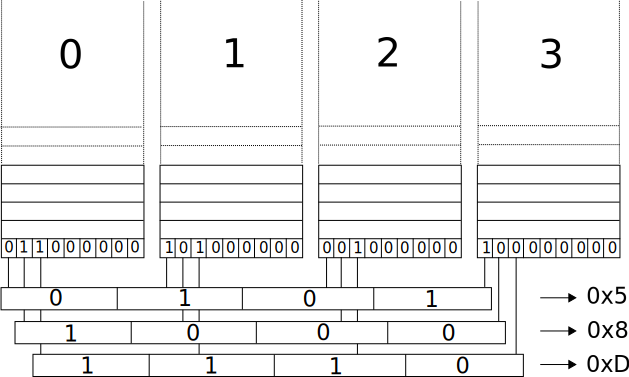
\includegraphics[width=\textwidth]{imgs/drawings/mode12h.pdf}
\caption{Banks layout in mode 12h.}
\end{figure}
\par

The only good thing about this mode is that it has square pixels: The aspect ratio 640x480 matches the 4:3 of a CRT so there is no distortion of the framebuffer when it is ouputed to the screen.\\
\par

Pretty much everything else is bad:\\
\begin{itemize}
\item NO double buffer: 640X480/2 = 0x25800 bytes which is more than half the 256KB (0x40000) of VRAM available.
\item The high resolution of Mode 12h is actually a drawback for a 3D engine: More pixels meant more calculations and more drawing.
\item 16 colors looks really, REALLY ugly.
\end{itemize}

 \begin{figure}[H]
\centering
 \fullimage{wolf3d_ega.png}
 \caption{Wolfenstein3D in 16 colors}
\end{figure}





 
  \subsection{VGA Programming: Mode 13h}
  Mode 13h is far more appealing since it offers a lower resolution with 256 colors. It also has the advantage of faking linear buffer: A special chip called Chain-4 uses the lower 2 bit of the RAM address to match it in the VGA RAM:\\
  \par
 \begin{figure}[H]
\centering
      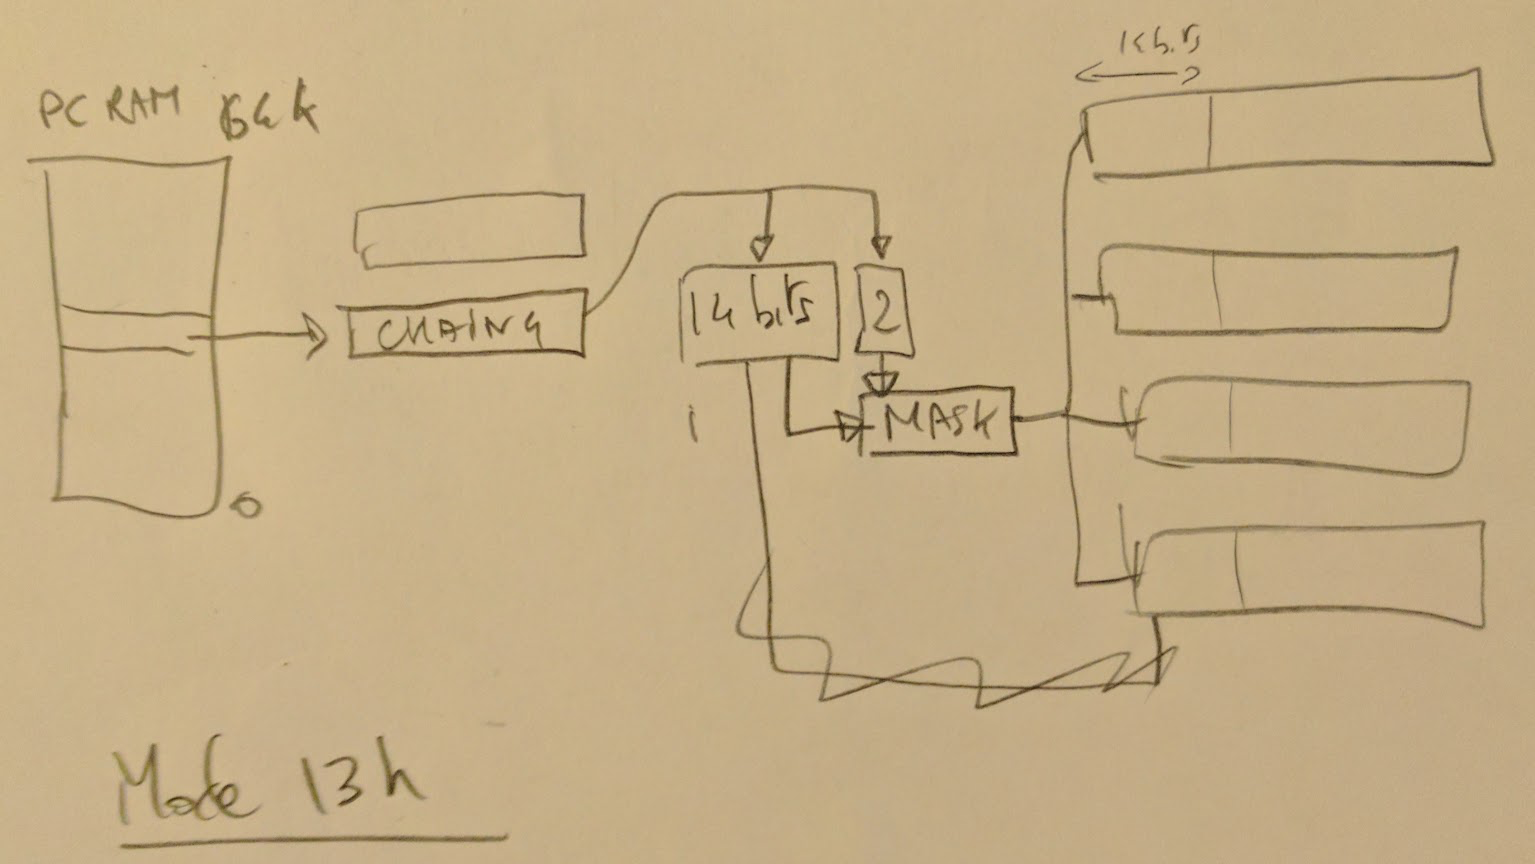
\includegraphics[width=\textwidth]{imgs/drawings/mode_13h.pdf}
\end{figure}
\par

When writing or reading at an address K in RAM, the Chain-4 breaks down that address in two parts:
\begin{itemize}
\item The 2 low bits are used to configure the mask automatically. Hence 0x00 goes to bank 0, 0x01 to bank 1 and so on.
\item The 14 high bits are switched right by two bits and used as offset in the bank.
\end{itemize}
  \par
  For example, writing at 0x0AF11 would result in writing in bank 3 at offset 0x0AF. Since this is all hardwired it is fast and framebuffer could be refreshed at 70Hz.
 \begin{figure}[H]
\centering
      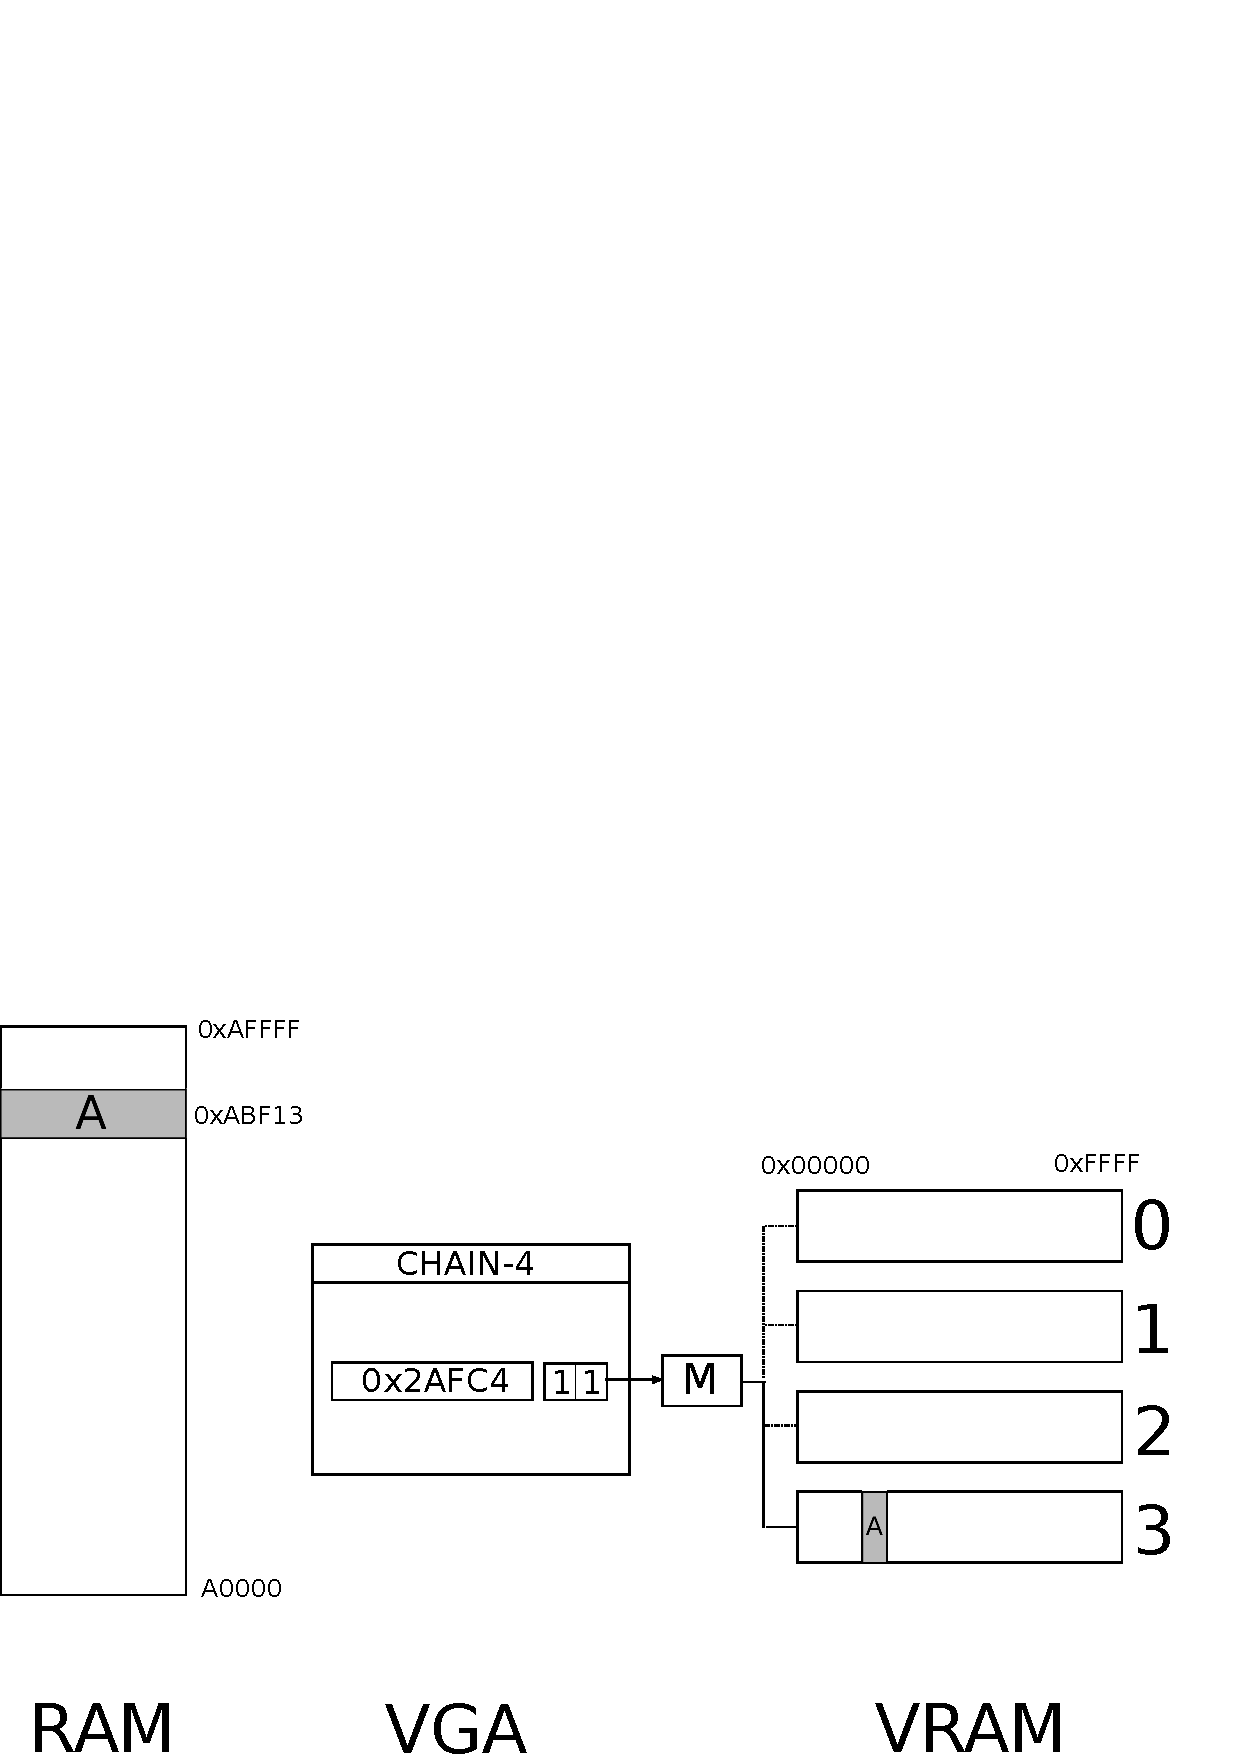
\includegraphics[width=\textwidth]{imgs/drawings/mode_13h_example.pdf}
\end{figure}
\par
The side effect is that 75\% of the RAM is wasted (since only 14 bits were usable for offset).\\

  \par
  To setup the VGA in Mode 13h using the BIOS is incredibly easy:\\
  \par
  \lstinputlisting[ language={[x86masm]Assembler}]{code/vga_mode13.asm}
  
  
  The \codeword{int 10} is a software interrupt call to the BIOS routine in charge of Graphic setup. It looks up the \codeword{ax} register to setup all 300 VGA register with the corresponding mode. After the VGA is initialized one can write to the mapped 0xA000 e.g: Clear the screen to black:\\
  
  \begin{minipage}{\textwidth}
  \lstinputlisting[language=C]{code/clear_vga.c}
  \end{minipage}
  
  Mode 13h looks a bit better than 12h but it is in fact also terrible for game or even photos:\\
  \begin{itemize}
\item With Chain-4, all the RAM address space is used and there is no way to have a double buffer.
\item Since the resolution is 320x200, the aspect ration (1.6) does not fit the monitor (which is 1.5). As a result the image is stretched when transfered from the 
framebuffer to the CRT.
\end{itemize}

\begin{figure}[H]
  \centering
  \fullimage{circleframebuffer.png}
  \caption{Drawing a circle in the framebuffer}
\end{figure}

\begin{figure}[H]
  \centering
  \fullimage{circlescreen.png}
  \caption{How the framebuffer looked once stretched on the CRT monitor :( !}
\end{figure}
\par





\subsection{The importance of doublebuffering}
Double buffering is paramount for smooth animation. With only one buffer the software has to work exactly at the frequency of the CRT (70Hz). Otherwise a phenomenon known as "tearing" appears. Let's take the example of an animation rendering a circle moving from the left to the right:
\par
\begin{figure}[H]
\centering
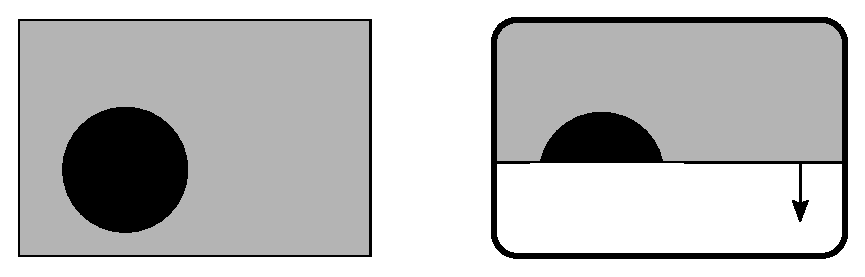
\includegraphics[width=\textwidth]{imgs/drawings/doublebuffer_before.eps}
\end{figure}
\par
In this example the CPU has finished writing the framebuffer (on the left) and the CRT (on the right) electron bean has started to scan it onto the screen. At this point in time the electron bean has scanned half the framebuffer and therefore the circle has been partially drawn on the screen.
\par
\begin{figure}[H]
\centering
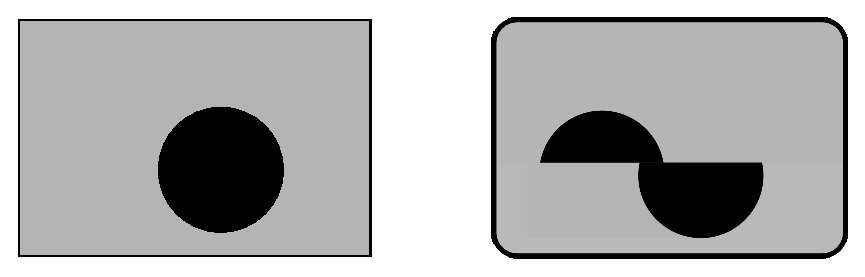
\includegraphics[width=\textwidth]{imgs/drawings/doublebuffer_after.eps}
\end{figure}
\par
But if the CPU is fast eonugh (faster than 70Hz), it can write the framebuffer again, before the scan is completed. This is what happened here: The next frame was drawn with the circle moved to the right. The electron bean did not know what and just kept on scanning the framebuffer. The result on screen is now a composite of two frames: It looks like two frames were torn and tapped together. Hence the name "tearing".\\
\par
With two buffers (a.k.a double buffering) the CPU can start writing in the second framebuffer without messing with the framebuffer being scanned to the screen\footnote{Now the CPU speed is capped by the CRT refresh rate. Triple buffering can solve this at the price of frame latency.}. No more tearing!
















\section{Audio}
A PC came equipped with a beeper, commonly known as a "PC Speaker" capable of generating square wave via only 2 levels of output:\\
\par
 \begin{figure}[H]
\centering
\includegraphics[width=\textwidth]{imgs/drawings/square_wave.pdf}
\caption{Two beeps of different frequencies generated via PC Speaker.}
\end{figure}

\par
 The purpose of this primitive loudspeaker was to signal hardware problems at runtime with beep codes:\\
\par
\begin{tabularx}{\textwidth}{l l}
\textbf{Beep Code} & \textbf{Meaning}  \\ \hline
No Beeps                         & Short, Bad CPU/MB, Loose Peripherals \\ \hline
One Beep                         & Everything is normal\\ \hline
Two Beeps                        & POST/CMOS Error \\ \hline 
One Long Beep, One Short Beep    & Motherboard Problem \\ \hline
One Long Beep, Two Short Beeps   & Video Problem \\ \hline
One Long Beep, Three Short Beeps & Video Problem \\ \hline
Three Long Beeps                 & Keyboard Error \\ \hline
Repeated Long Beeps              & Memory Error \\ \hline
Continuous Hi-Lo Beeps           & CPU Overheating \\ \hline
\end{tabularx}\\
\bigskip
\par
Needless to say one tune was not usable for anything. But some peoples had started to see a market and they were companies manufacturing what were known as "sound cards". You could buy them separatately and insert them into one of the ISA slot of the machine. These cards could be connected to real audio speakers via 3.5mm jack and tremendously improve the sound capabilities. In 1991, three companies competed to become the dominant sound card: Adlib, Creative and Disney drawing a small eco-sytem of four cards:\\
\par
\begin{itemize}
\item Adlib music card.
\item SoundBlaster 1.0 (Mono).
\item SoundBlaster Pro (Stereo).
\item Disney Sound Source.
\end{itemize}
\par
Even though adoption was improving, a fast majority of PCs had no sound cards which once again was a huge problem for game developers.


  \subsection{AdLib}
  Started by Martin Prevel, a former professor of music in 1988. After an initial struggle to convince game developers to use their card, Adlib had convinced Sierra On-Line to support their hardware for their lates title: King's Quest IV (over 3 million copies sold). Soon, all game developers embraced the Adlib. Equipped with a Yamaha YM3812 also known as the OPL2 the card can produce 9 channels of sound, each made of two oscillators or 6 channels with 5 percussion instruments available. The FM synthetiser was limited but allowed to play pleasant musics.\\
  \begin{figure}[H] \centering 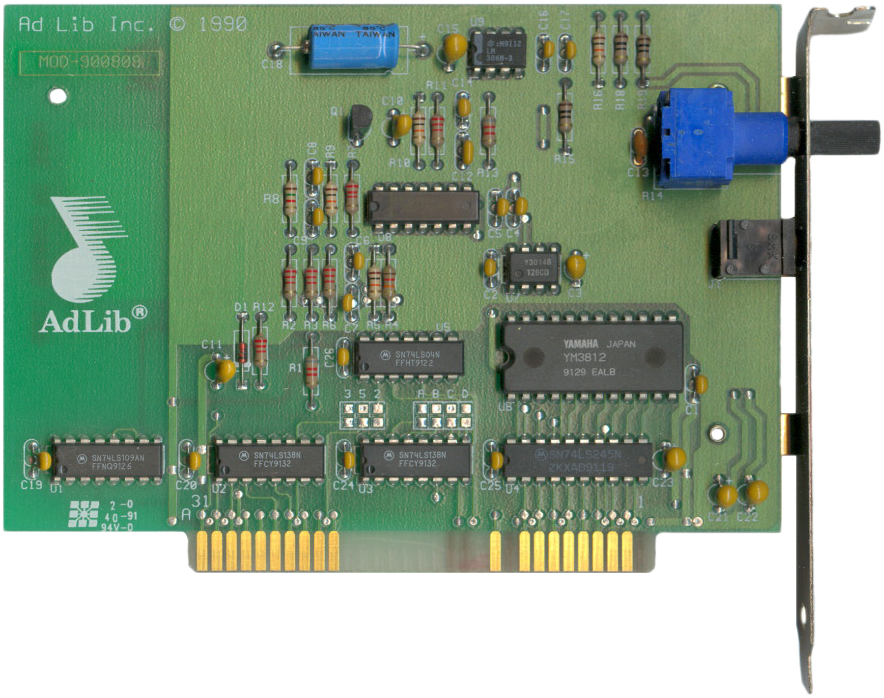
\includegraphics[width=\textwidth]{screenshots/hardware/adlib.png} \end{figure}
   \bu{Trivia :} Notice the 8 bits ISA bus connector at the bottom.
\par
\bu{Trivia :} Canadian company and especially Quebec were very innovative in the early 90s. Ad Lib manufactured Sound Card, Matrox made a killing with Millenium Graphic Card, Watcom the best DOS C compiler which would be used for Doom. ATI\footnote{History would repeat itself in the late 90s in the field of Graphic Cards: Nvidia Vs ATI} would later emerge as AAA GPU manufacturer in the years 2000.\\
  
  


  \subsection{Sound Blaster}
  The Sound Blaster 1.0 (code named "Killer Kard"), was released in 1989 by Creative labs. It was a smart product which clearly came after Adlib dominant position. Not only they were equipped with the same OPL2 chip, prodiving 100\% compatibility with Adlib musics playback, they were technologically superior with a DSP\footnote{An Intel MCS-51 market as a "Digital Sound Processor", not "Digital Signal Processor"}  allowing PCM playback (digitized sounds) at 8 bits per sample and 23Hz. The card also came with a DA-15 port allowing connection of a joystick!. That is right: The only way to connect a joystick to a PC was to buy a sound card\footnote{In the late 90s the only way to have a CD-ROM reader was also to buy a soundcard}.\\ 
\par

\begin{figure}[H] \centering 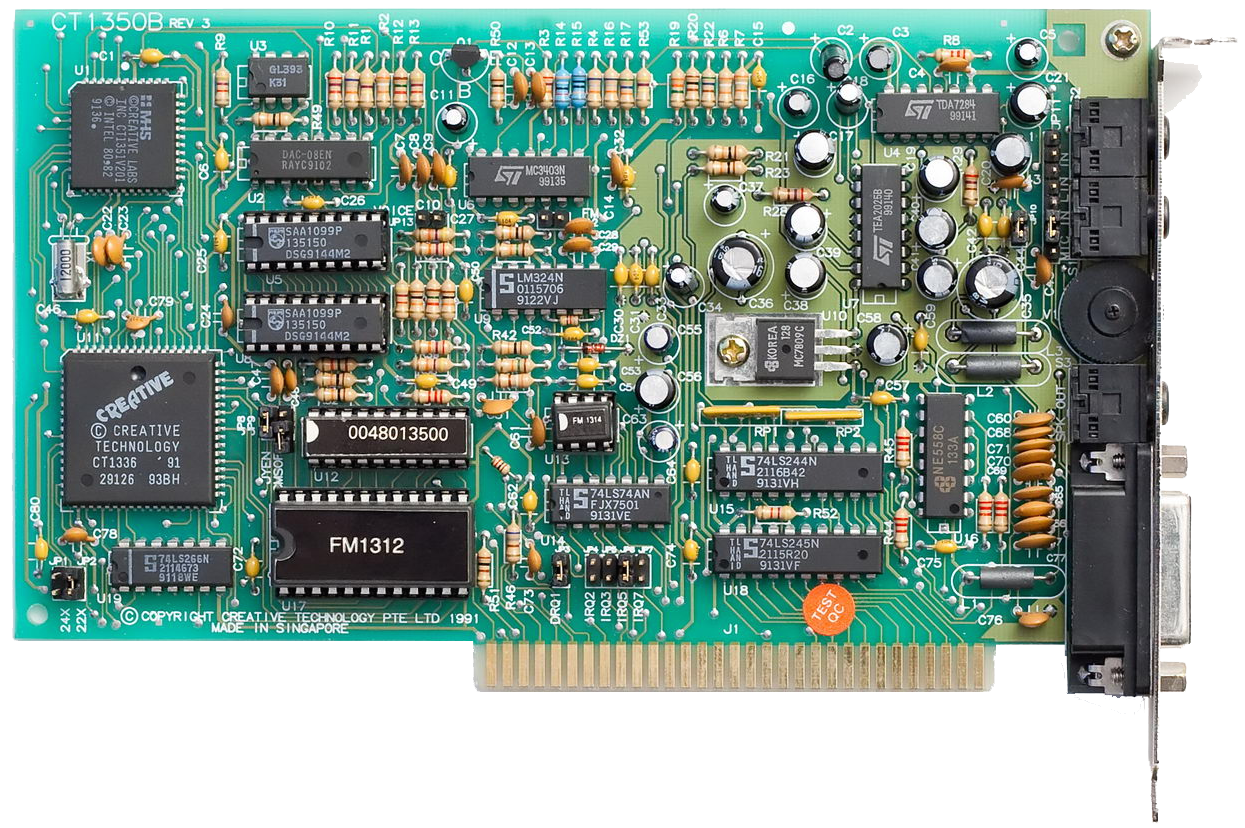
\includegraphics[width=\textwidth]{screenshots/hardware/sb.png} \end{figure}
\bu{Trivia :} Notice the 8 bits ISA bus connector at the bottom.\\
  \bu{Trivia :} The quality of the card would lead the Sound Blaster to become a de-factor standard in the 90s annd bring Adlib to bankruptcy\footnote{The reign of the Sound Blaster came to an end with Windows 95 which standardized the programming interface at application level (eliminating the importance of backward compatibility with Sound Blaster)}.


  \subsection{Sound Blaster Pro}
The Sound Blaster Pro had all the capabilities of a Sound Blaster 1.0 but also supported faster digital input and output sampling rates (up to 22.05 kHz stereo or 44.1 kHz mono), added a "mixer" to provide a crude master volume control (the round thing on the picture), and a crude high pass or low pass filter. It used a pair of YM3812 chips to provide stereo music-synthesis (one for each channel).\\
\begin{figure}[H] \centering 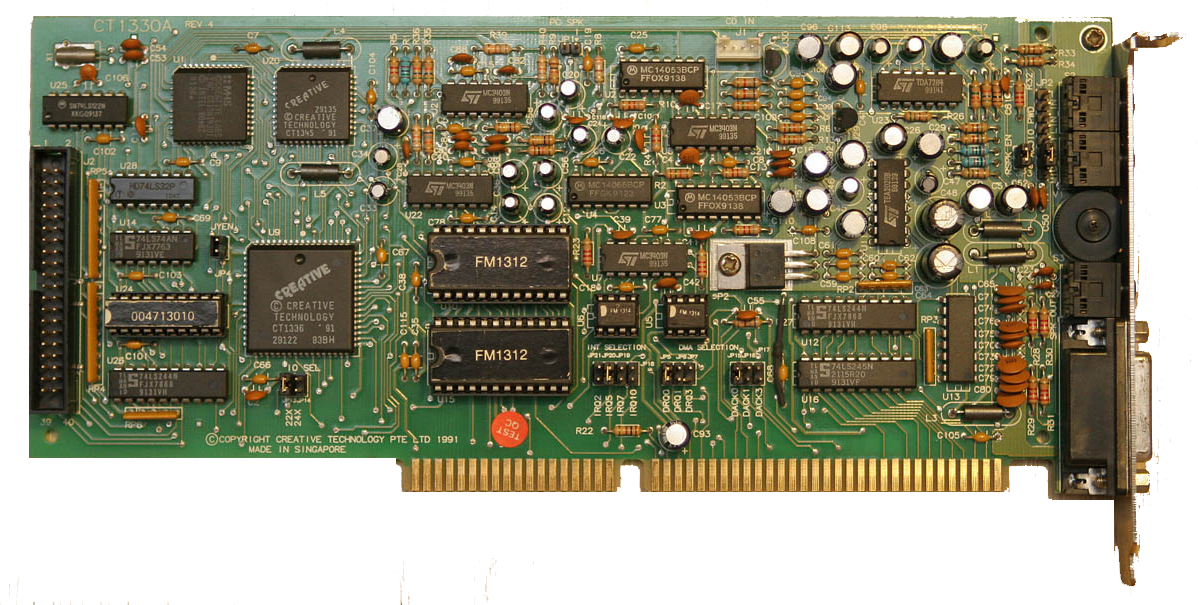
\includegraphics[width=\textwidth]{screenshots/hardware/sbpro.png} \end{figure}
\bu{Trivia :} The card appears to have a 16 bits ISA bus connector (check the difference with Sound Blaster 1.0. However it does not have 'fingers' for data transfer on the higher "AT" portion of the bus connector. It uses the 16-bit extension to the ISA bus to provide the user with an additional choice for an IRQ (10) and DMA (0)m channel only found on the 16-bit portion of the edge connector.)\\
\par
\bu{Trivia :} Notice on the very left of the card in black a CD-ROM interface. The only way to connect a CD-ROM to a PC back then.


  \subsection{Disney Sound Source}
  Plugged into the printer port (parrallel port) of the PC. Covox-idea based DAC, marketed by Disney Software in early 1990s. It consisted of 2 parts: a DAC plugged into printer port and separate amplifier / speaker box.[5] Its price was set to only \$14 and it was originally supported by many games. It used external power (9 volt battery) and could be turned on/off by software.\\
  \par
  \begin{figure}[H] \centering 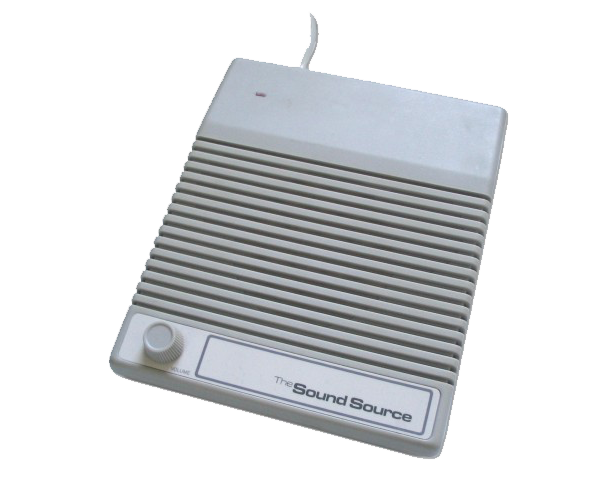
\includegraphics[width=\textwidth]{screenshots/hardware/ss.png} \end{figure}








\section{Inputs}
A time before the ubiquitous USB, inputs were a mess with no less than four ports, all programed with different I/O addresses.\\

The parallel port (DB-25) was on every computer and usually used mostly to connect matrix printers (loud thing that printed with needles). The parallel port was multipurpose: The Disney Sound Source could be plugged into it and generate crude sounds. The slow bandwidth of the port (150 kbit/s) forbid anything too melodious.\\
 \begin{figure}[H]
\centering
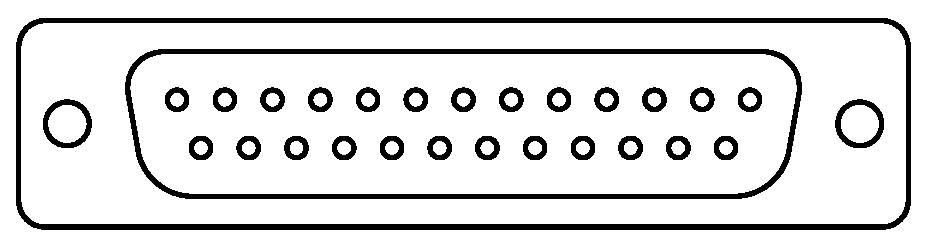
\includegraphics[width=0.3\textwidth]{imgs/drawings/ports/DB-25_parallel_port.eps}
\caption{Parallele Port}
\label{fig:parallelPort}
\end{figure}


The serial port (DE9) was used to connect the mouse:
 \begin{figure}[H]
\centering
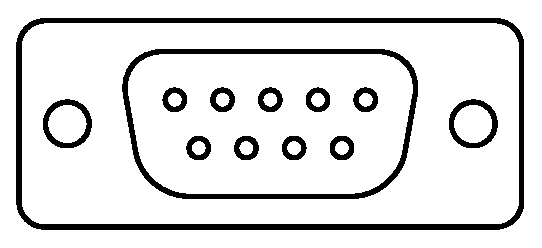
\includegraphics[width=0.15\textwidth]{imgs/drawings/ports/DE9_serial_port.eps}
\caption{Serial Port}
\label{fig:serialPort}
\end{figure}

The PS/2 port was used to connect a keyboard:
 \begin{figure}[H]
\centering
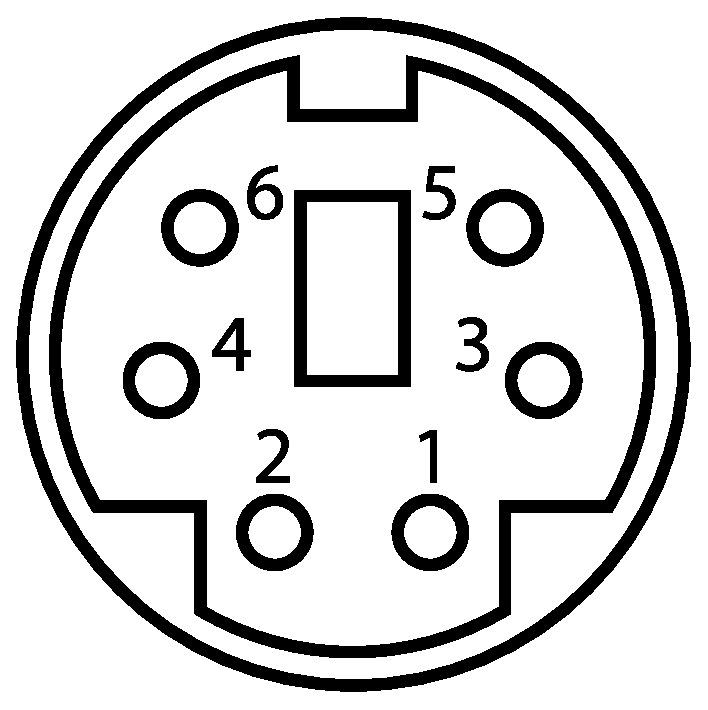
\includegraphics[width=0.07\textwidth]{imgs/drawings/ports/MiniDIN-6_PS2.eps}
\caption{PS/2 Port}
\label{fig:ps2Port}
\end{figure}


Finally, the sound card connected via the ISA bus provided a new port: A Game Port (DA-15) allowing to connect a joystick:
 \begin{figure}[H]
\centering
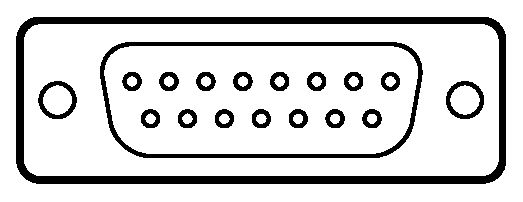
\includegraphics[width=0.19\textwidth]{imgs/drawings/ports/DA-15_GamePort.eps}
\caption{Game Port}
\label{fig:gamePort}
\end{figure}

Note that without a sound card you were unable to connect a joystick !


\section{Bus}
Altought developers had no control over it, it is still worth mentioning how these component are connected together via the Northbridge and Southbridge chipsets:\\ 
\par
\begin{figure}[H]
\centering
      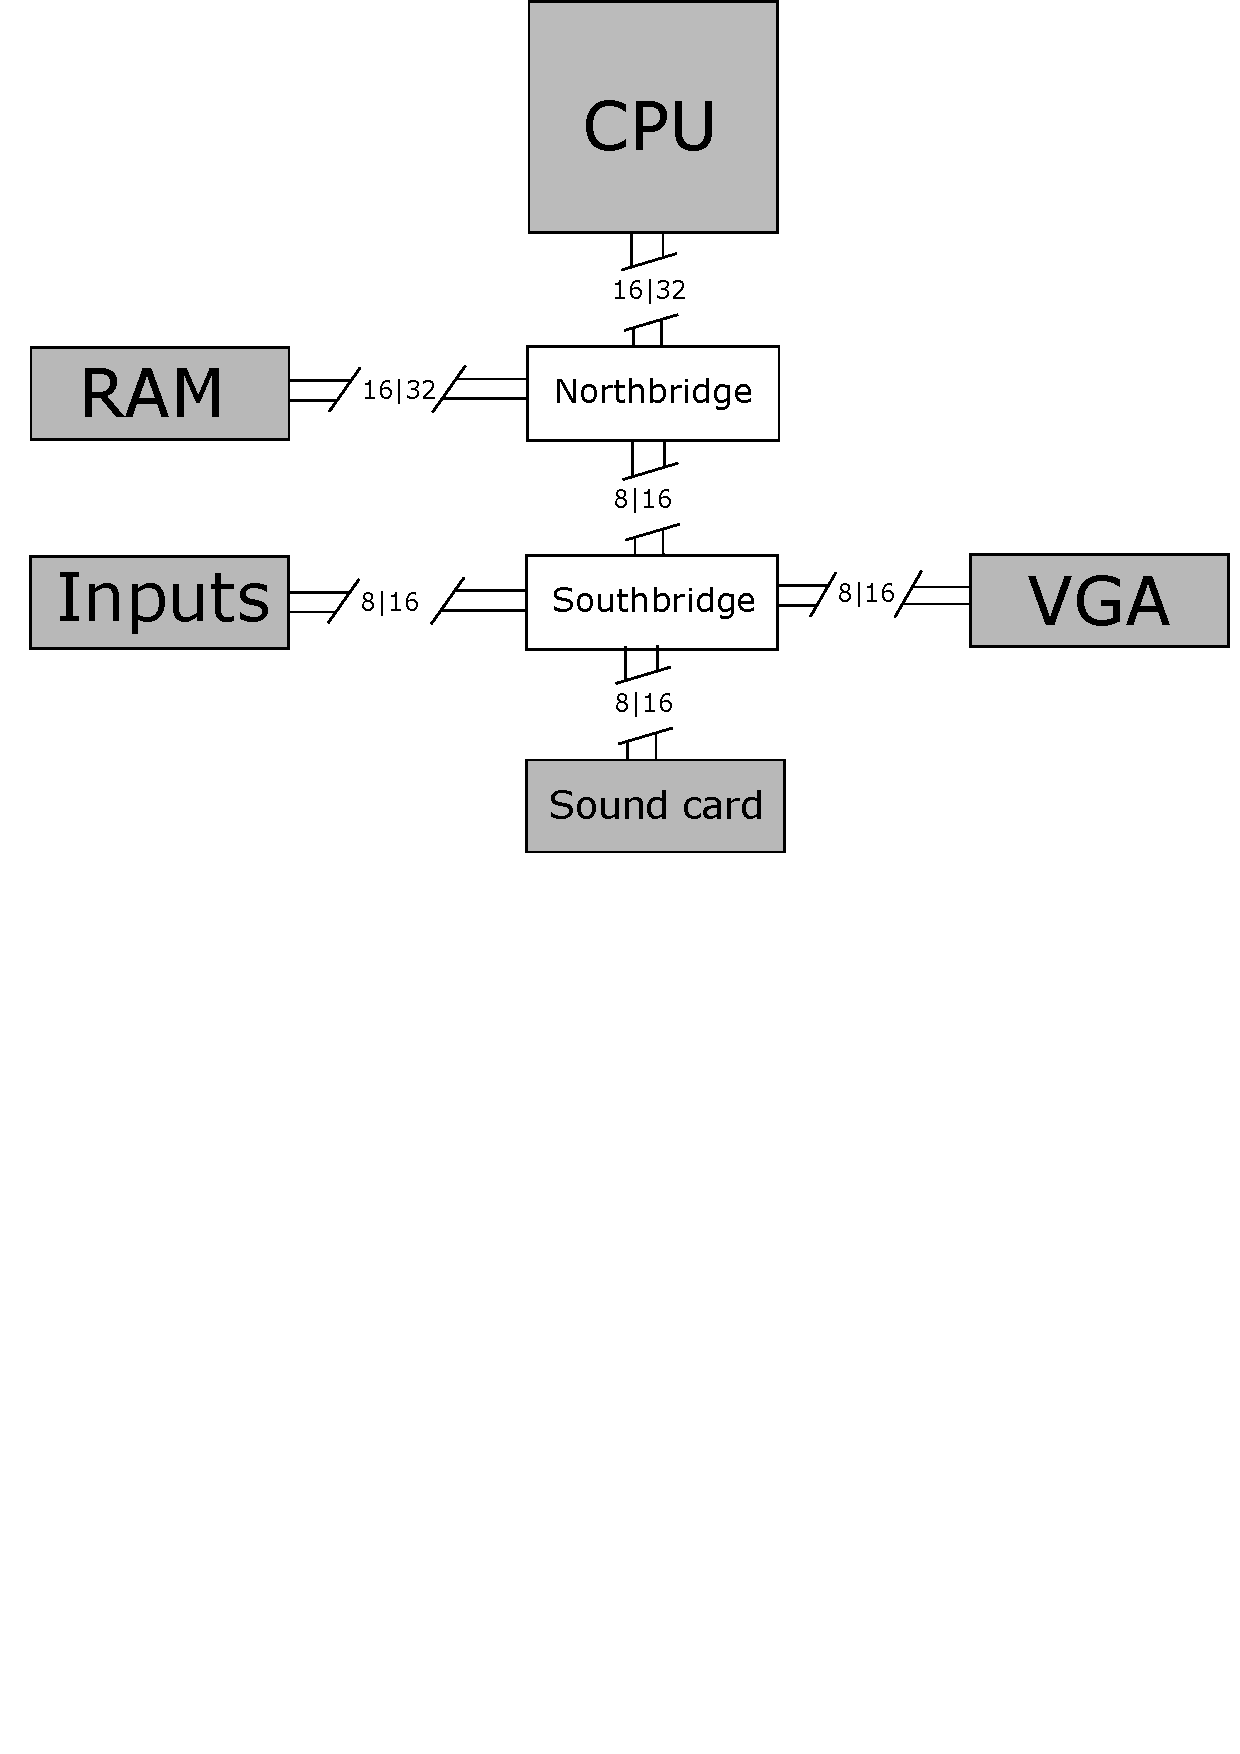
\includegraphics[width=\textwidth]{imgs/drawings/bus.pdf}
\end{figure}
\par
The Northbridge connecting the CPU to the RAM is 16 bits wide on 286 and 386SX but 32 bits wide on 386DX machines. It runs at the same speed as the CPU.\\
\par
The Southbridge run on ISA\footnote{Industry Standard Architecture}. Invented in 1981, it can offers either:
\begin{itemize}
\item 8-bit data bus at 4.77 MHz  for 19.1 Mbit/s
\item 16-bit data bus at 8.33MHz for 66.7 Mbit/s\footnote{https://en.wikipedia.org/wiki/List\_of\_device\_bit\_rates} bandwidth.
\end{itemize}
The width of the data bus depends on how many "fingers" a card has.\\
\par

 In practice, due to packet overhead and interrupts, the effective bandwidth of the bus is divided by two. As a result, a PC equipped with an 8-bits ISA VGA card can push 19.1Mbits/s/2 = 1.5MB/s. In Mode 13h, a frame is 320x200 bytes = 64,000bytes. The theoretical maximum framerate with a CPU taking 0ms to render a frame is 1,500,000 / 64,000 = 23 frames per seconds.\\
 \par
 On a 16 bits VGA card, 33,400,000 bits per seconds gives 33,400,000/8/64000 = 65 frames per seconds.\\
 \par
 If you factor in other things which had to transit on the bus such as palette, keyboard interrupt, mouse inputs and music/sounds (at 23kHz sampling a digitized sound effect consumes 23,000/70 = 328 bytes per frame) you understand well why no PC of the era could max out the VGA's 70 frame per seconds. The best demos and games usually reached 35 frames per seconds.


\section{Summary}
In a nutshell, to say a PC was difficult to program for games would be an understatement. The CPU was good at doing the wrong thing, the best graphic interface allowed neither double buffering nor square pixels, the memory model only allowed 1 standard MB...with address composed of two separate 16 bits registers. Last but not least the default sound system allowed only one tune...and the people who did have a sound card made an eco-system of four overlapping configurations. Yet, despite all these unfavorable conditions, teams of developers gathered to tame the beast and unleash its power to gamers. One of them was Ideas from the Deep, also know was id Software.
\end{document}




